\chapter{Ion Trap Apparatus}
\minitoc
% Main points:
    % Give a working overview of the apparatus.
    % The desired audience here is 
        %   i) Future members of FastGates, 
        %  ii) Anyone building a similar experiment, 
        % iii) Readers of other chapters who want technical detail of the apparatus.
    % Block diagram of the system
% Pre reqs:
    % Motivation for why we want this apparatus!

    % print linewidth
    After 70 years of ion confinement development (since the quadrupole mass
    spectrometer in the 1950s~\cite{paul_electromagnetic_1990}), and the myriad
    use-cases from time standards, to analytic chemistry, to quantum computing,
    there are naturally many systems and thesi apparatus chapters in existance
    today. As such, we structure this chapter in the following way: 
    Following on from the standard requirements of an ion trap system, provided in the introduction section~\ref{sec:Intro Ion trap},
    we discuss the unique motivation and design specifications of our system; 
    We then present an abstract schematic of the system in
    its current form, highlighting the constituent subsystems, and the optical
    and electrical signal paths; 
    The remaining sections of the chapter contain
    the technical detail, perhaps more relevant to the practicing experimental
    student, and the hardware enthusiastic.\\

\section{Specification}
\label{sec:Spec}
% Main points:
    % Block diagram of the system
    Ion-trap experiments are exceptionally versatile in their application, however in the vast search space of quantum-information applications, we want a system particularly tailored for three avenues of study: 
    \begin{enumerate}
        \item Error channels on multi-qubit chains.
        \item Continuous variable quantum computing and simulation utilising the spin and motional degrees of freedom of the confined ions.
        \item Fast two-qubit entangling gates via phase stabilised optical standing waves.
    \end{enumerate}
    These latter two research directions were explored within our group on a
    previous apparatus, leading to state-of-the-art two-qubit entanglement rates
    on the ion trap platform~\cite{schafer_fast_2018,saner_breaking_2023}, creation
    of highly non-classical motional
    states~\cite{bazavan_squeezing_2024,saner_generating_2024}, and a simulation of
    Z2 gauge theories encoded via the spin and motional degrees of freedom of a
    two-ion chain~\cite{bazavan_synthetic_2023, saner_real-time_2025}. However, hard
    limitations of both scaling these demonstrations to longer ion chains, and
    of interaction strength due to availible optical intensity, were often
    restrictive. To solve both these issues, a new apparatus has been designed,
    constructed, and characterised, motivated by these applications. Colloquilly
    the system is named \textit{``FastGates''}, owing to its
    experimental objectives, and we shall refer to it as such throughout this
    chapter. \\
    These objectives give the following specific control requirements:
    \begin{itemize}
        \item Storage of medium length (5-10) qubit registers, section~\ref{sec:The Ion Trap}.
        \item Individual internal state control of each qubit, section~\ref{sec:Single Addressing System}.
        \item Stable motional modes for storing quantum information, section~\ref{sec:Trap RF Chain}.
        \item Dual high numerical apperture (NA) optical access for high-intensity standing waves, section~\ref{sec:Vacuum System}.
    \end{itemize}
    As the lifetime of such an apparatus extends past a single PhD generation,
    this thesis serves as a point-in-time description of the system, and where
    applicable, the planned future extensions will be highlighted as such. An
    abstract schematic of the current configuration is shown in
    figure~\ref{fig:apparatus} with blocks resembling either electronic,
    mechanical, or optical subsystems.

    \begin{figure*}
        \begin{center}
        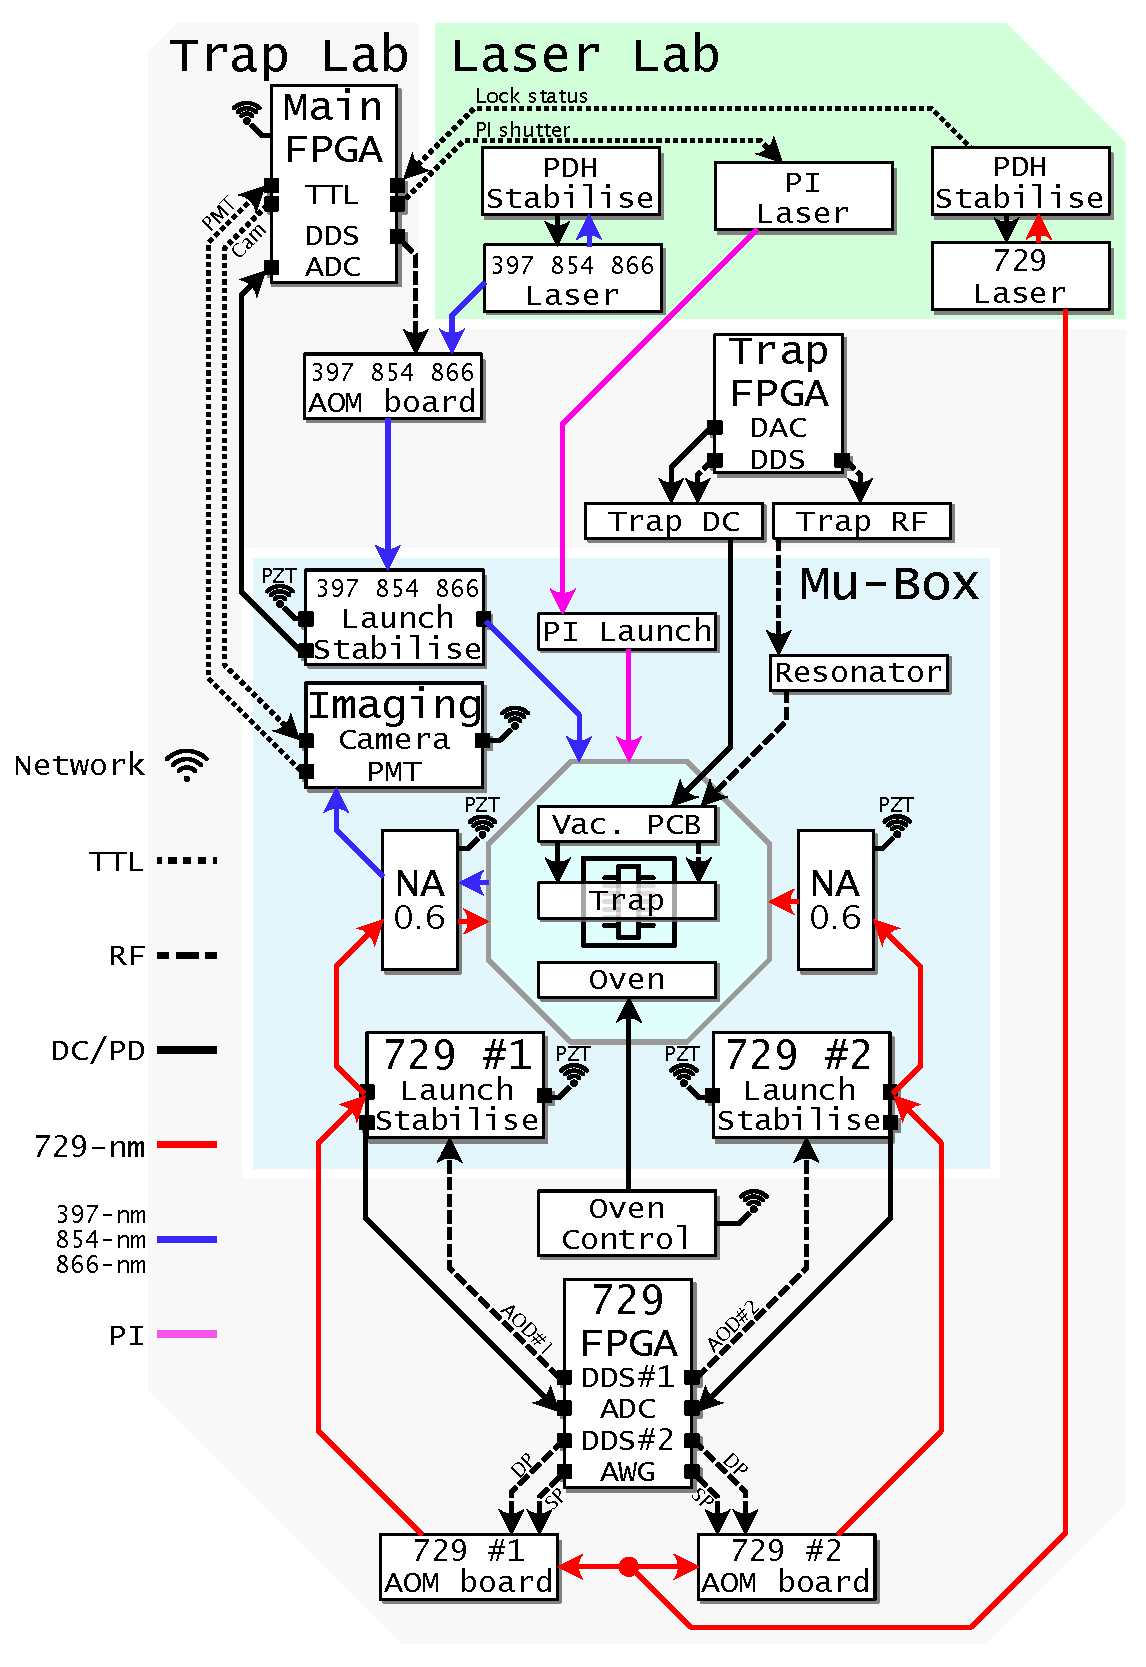
\includegraphics[width=\linewidth]{figures/pdf_figure/ch2/schematic_v2.pdf}
        \caption{Block diagram schematic of the \textit{FastGates} apparatus.
        Blocks resemble discrete subsystems, which shall be discussed within
        this chapter. Lines resemble relevant optical (free-space or in-fibre),
        RF, DC, and communication paths between subsystems.
        Block location signifies whether the device is in-vacuum,
        within the magnetic shielded (MuMetal) box, within the ``trap-lab'', or
        within the ``laser-lab''.  }
        \label{fig:apparatus}
        \end{center}
    \end{figure*}

\section{The Ion Trap}
\label{sec:The Ion Trap}
% Main points:
    % Introduce the NPL trap chip and its advantages
    % Short intro into the parts of the ion trap DC/RF fields.
    % Trap package CAD
    % Solidworks models of CAD with labels
    % Construction and S11 measurements of electrodes
    % Fastino channels
    % Experimental parameters for stable trapping
    % Quote the values we use for trapping/experiment
% Pre reqs:
    % Motivation for trapping an ion!

    \begin{figure}
        \begin{center}
        \noindent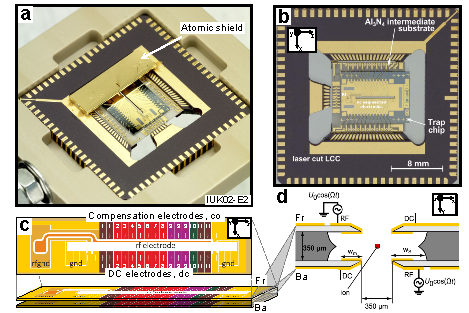
\includegraphics[width=\linewidth]{figures/pdf_figure/ch2/NPL_trap.pdf}
        \end{center}
        \caption{
            Schematics of the \emph{NPL} trap chip used in this experiment.
            \textbf{a)} A photograph of the trap chip used in the \emph{FastGates} experiment before being placed under vacuum. The top ``atomic shield'' can be seen here.
            \textbf{b)} A front view of the trap chip. Axial confinement is provided by a subset of the segmented DC electrodes. Radial confinement is provided by the RF rails. The trap chip and leadless chip carrier (LCC) are highlighted.
            \textbf{c)} A schematic of the electrode geometries and labelling for the front-face of the trap chip. A similar arrangement exists for the back-face however with the RF rail on the diagonally opposite electrode.
            \textbf{d)} A slice view of the trap. The red point here represents the ions, the gold are the RF and DC electrodes, and the grey is the silica substrate. It can be seen that the ion is $350\times\sqrt{2}/2 \simeq 250 \mu$m away from the nearest electrode. The numerical aperture of the ion plane due to the electrodes is $\sim 0.71$.
            Figures b) and d) adapted from Ref.~\cite{choonee_silicon_2017}, other panels adapted from private communication with the \emph{NPL} team.
        \label{fig:trap}}
    \end{figure}

    Recently, the micro-fabricated surface style linear Paul trap has gained
    popularity due to the maturity of chip fabrication
    technologies~\cite{allcock_surface-electrode_2011} and the potential route
    to scalability this offers. In the surface trap, the 3D radial and axial
    electrodes of a ``macro'' trap are effectively projected onto a 2D surface.
    The stable confining point of such a trap is typically designed to be on the order of $50-100~\unit{\micro\meter}$
    above the chip surface. The maturity of chip fabrication has enabled
    the manufacturing of complex multi-zone devices with many DC electrodes, amenable to ion shuttling~\cite{kaushal_shuttling-based_2020, sterk_closed-loop_2022}, and hence furthering progress towards Quantum CCD
    type architectures~\cite{kielpinski_architecture_2002}. However, this
    surface style geometry typically comes with two costs: the depth of the
    trapping potential is often greatly reduced due to anharmonicity~\cite{home_normal_2011}, and the close proximity of the
    surface to the ion can be a large contributor to motional heating
    rates~\cite{wineland_experimental_1998, turchette_heating_2000, brownnutt_ion-trap_2015, boldin_measuring_2018}. \\
    Our trap, provided by the \emph{National Physical Laboratory} in the UK,
    brings together the
    advantages of chip fabrication as well as the low heating rates and high
    trapping depths of a macro 3D style trap
    through utilising a micro-fabricated 3D trap geometry with greater ion-surface distances than typical planar traps.
    Details on its design and characterisations can be found in Ref.~\cite{see_fabrication_2013,
    wilpers_monolithic_2012, choonee_silicon_2017}. Figure~\ref{fig:trap} shows the electrode geometry of the trap and the relevant length scales.
    The trap package consistes of an outer leadless chip carrier (LCC) with outer
    pads routing DC, RF, and ground connections to an intermediate
    Al\textsubscript{3}N\textsubscript{4} substrate. The connection to the front
    and back surfaces of the trap chip is made through vias and wire bonds to
    the intermediate substrate~\cite{wilpers_compact_2013}. The trap chip 
    is a monolithic double-sided silicon device with gold plated electrodes on
    the front (Fr) and back (Ba) surfaces. These two layers are shown
    schematically in the bottom panel of $(c)$. The electrode schematic for the
    front surface is shown, and the electrode indexing convention is
    highlighted. Electrodes recessed from the ion due to the RF rail are named
    ``compensation''-electrodes (co), while electrodes on the opposite side
    provide the strong DC potential required for axial
    confinement\footnote{Note: Compensation electrodes co1 and co11 on both
    front and back surfaces are grounded on the trap package, and so are not
    available for use. There is a continuity fault on front dc11 and so this
    electrode is also not available for use.}.
    We typically
    trap ions centered on electrode dc5. Panel $(d)$ shows a slice view of the
    trapping region, highlighting the ion position between the front and back
    surface electrodes. The dual RF rails and DC electrodes are shown in gold,
    and the undercut silicon bulk is highlighted in dark grey.\\
    The next two subsections describe the source of RF and DC voltages to the trap
    electrodes. The physical mounting of the trap in the vacuum system is
    discussed in section~\ref{sec:Vacuum System}, and the optical access to the
    trap is discussed in section~\ref{sec:Vacuum System}.\\
    %Figure like Milne would be nice here - but showing zig-zag for 5 ions is hard...
    % Giving details of trap potentials, frequencies, and voltages in a table would be nice

\subsection{Trap RF Chain}
\label{sec:Trap RF Chain}
% Main points:
    % Maybe a figure describing the elements within the RF chain
        % Frequency source (Urukul)
        % Resonator
        % RF rails
    % Quote values we use.
% Pre reqs:
    % NPL trap geometry
% Figures
    % Block diagram of the RF chain with values for each element.
    % Q factor of the resonator
    % Central frequency using ion

    To utilise radial motional modes for low error quantum gates, we require the
    radio frequency (RF) field that produces the desired trapping
    pseudopotential to be both frequency and amplitude stable. Furthermore, as the natural time scale for two-qubit gate durations is $\tau = 2\pi/\omega_m$ (see section~\ref{sec:Geometric Phase Gates}), where $\omega_m$ is the motional mode angular frequency, then greater motional mode frequency is desired for fast entanglement.
    From equation~\ref{eqn:pseudo_pot}, it can be seen that radial motional mode frequency is proportional to RF voltage, and inversely proportional to the frequency.
    The \emph{NPL} trap used in the \emph{FastGates} apparatus is rated for a max peak-to-peak voltage of $400$~Vpp on the RF
    electrodes. To target high motional mode frequencies, saturating this maximum voltage is desirable, however, for safe operation, typically the trap is provided a maximum RF voltage $V_{RF}=360$~Vpp.
    % See OneNote 2026-05-18 13.35 dBm +17 dB = 30.35 dBm -> 20.8 Vpp
    % See Onenote 2023-10-24 20 pF Capacitance
    The RF chain which provides this signal is schematically shown as:
    \begin{center}
        \noindent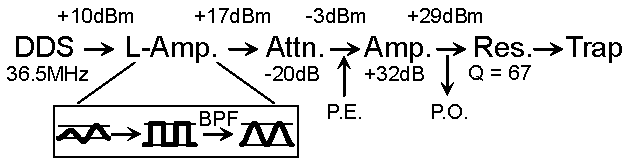
\includegraphics[width=0.6\linewidth]{figures/pdf_figure/ch2/rf_chain.pdf}
    \end{center}
        % \caption{Schematic of the RF chain. The RF signal is generated by a DDS, passed through a non-linear voltage clamp to suppress AM noise, amplified by a low-noise amplifier, and then impedance matched to the trap electrodes through a custom resonator circuit. The resonator also provides some bandpass filtering of the RF signal.}
            %\label{fig:rf_chain}

    \noindent and embedded within the schematic~\ref{fig:apparatus}, beginning with the \emph{Trap FPGA}. Each element of the chain is designed to provide a low-noise, high-voltage RF signal to the trap electrodes, and is discussed in turn below.\\
    \begin{figure}
        \begin{center}
        \noindent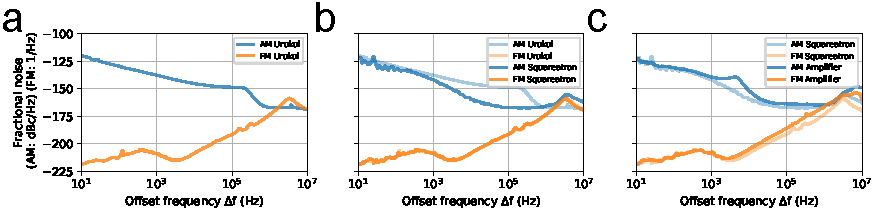
\includegraphics[width=\linewidth]{figures/pdf_figure/ch2/SSB_chain.pdf}
        \end{center}
        \caption{Characterisation of the RF chain. \textbf{a)} SSB spectra for AM and PM, given as fractional noise, measured after the \emph{Urukul}. \textbf{b)} Measured after the \emph{Squareatron}. \textbf{c)} Measured after the amplifier.}
            \label{fig:SSB_chain}
    \end{figure}
    \begin{figure}
        \begin{center}
        \noindent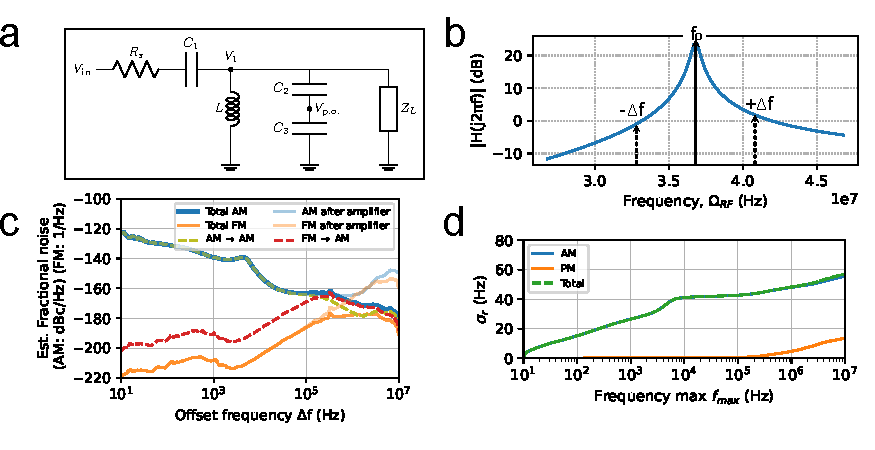
\includegraphics[width=\linewidth]{figures/pdf_figure/ch2/res_comb.pdf}
        \end{center}
        \caption{Expected SSB after the resonator, and estimated mode frequency noise. \textbf{a)} Resonator circuit diagram. \textbf{b)} Resonator lineshape, given by magnitude of the transfer function $|H(f)|$. \textbf{c)} Expected AM and FM fractional noise spectra after the resonator. \textbf{d)} Integrated RMS noise of radial motional mode frequency due to the RF chain.}
            \label{fig:res_H}
    \end{figure}
    The frequency source is a direct-digital-synthesiser (DDS), named \emph{Urukul}~\cite{kasprowicz_urukul_2022}, part
    of the \emph{Artiq Sinara}~\cite{kasprowicz_artiq_2020} hardware ecosystem. \emph{Urukul} is used extensively in our lab for driving acousto-optic modulators (AOMs) and here used as the source drive of our trap RF.
    The \emph{Urukul} is operated at maximum output power, $+10$~dBm, and with a frequency $\sim 35$~MHz (set by resonator, discussed below).
    As can be seen in equation~\ref{eqn:pseudo_pot}, amplitude and frequency instability will directly lead to radial mode instability.
    Expanding for small amplitude, $dV_{RF}$, and drive frequency, $d\Omega_{RF}$, errors we find the motional mode frequency, $\omega_r'$, is related to the ideal frequency, $\omega_r$, by 
    \begin{equation}
    \omega_r' = \omega_r(1 + dV_{RF}/V_{RF} - d\Omega_{RF}/\Omega_{RF}),
    \end{equation}
    where we can see both errors affect the motional mode frequency linearly.
    The instability of the oscillator can limit motional mode coherence time (see section~\ref{sec:Motional Coherence} for characterisation with the ion). We measure noise originating from both amplitude modulation (AM) and frequency modulation (FM) across the RF chain using a phase noise analyser\footnote{Rhode and Schwartz FSWP PNA}.
    This was done to verify low-noise operation of the individual devices, and to estimate expected motional mode errors due to the inherent noise on the RF chain. \\
    We quote FM as the fractional frequency stability power spectral density (PSD), 
    \begin{equation}
    S_y(f) = \frac{f^2}{f_0^2} S_{\phi}(f),
    \end{equation}
    where $S_{\phi}(f)$ is the phase noise PSD (which is the Fourier transform of the Autocorrelation function) $f$ is the offset frequency, and $f_0$ is the carrier frequency. $S_y(f)$ has units of
    $\left[\frac{1}{\unit{\hertz}}\right]$. AM noise is quoted as the single sideband (SSB) power, $S_\alpha$, in a 1~Hz bandwidth at an offset frequency, $f$, from the carrier, normalised to the total power of the carrier, and is here given in units of $\left[\frac{\mathrm{dBc}}{\unit{\hertz}}\right]$. \\
    Figure~\ref{fig:SSB_chain}, panel $(a)$ displays the \emph{Urukul} AM and FM spectra. The \emph{Urukul} is phase referenced to the master FPGA board (\emph{Kasli}), which is in turn phase locked to an external $10~\unit{\mega\hertz}$ atomic clock\footnote{\todo{ToDo: Abaqus atomic clock PN}}. It can be seen that AM noise dominates up $\sim 1$~MHz, suggesting that this will be the limiting error source for motional mode stability.
    The AM noise may be reduced by using a non-linear voltage clamp. We use an ``ultra-low noise limiting amplifier'' named
    \emph{Squareatron} developed previously in the group, and further refined by \emph{Oxford Ionics}. 
    \emph{Squareatron} takes an input RF signal and converts to a stable amplitude square-wave output which is subsequently bandpassed around the desired RF frequency to recover the sinusoidal signal, but with significantly reduced AM noise.
    The AM and FM after the \emph{Squareatron} is shown in panel $(b)$.
    It can be seen that between $1~\unit{\kilo\hertz}$ and $1~\unit{\mega\hertz}$, AM is considerably suppressed. There appears to be an increase in AM at higher frequencies \todo{ToDo: explore this further}. The \emph{Squareatron} has a $17$~dBm output power, which is attenuated by $-20$~dB before an amplification stage to reach the desired power for the trap. Highlighted in the above chain schematic is the option to input a parametric excitation signal (P.E.), which we shall discuss further in section~\ref{sec:Micromotion}. For the following measurements, the P.E. branch was removed.
    AM and FM introduced by the low-noise amplifier\footnote{Mini-Circuits ZHL-1-2W-S+}, can be seen in panel $(c)$. Most notably an increase in AM is seen between $1~\unit{\kilo\hertz}$ and $10~\unit{\kilo\hertz}$.\\
    To impedance match the 50~$\Omega$ line from the amplifier to
    the small capacitance  of the trap electrodes and vacuum feedthrough, a resonant 
    matching circuit is used.
    This ``resonator'' has three main effects on our system:
    \begin{enumerate}
    \item The source $50~\unit{\ohm}$ is matched to the (almost) purely capacitive load.
    \item The voltage step up provides the neccesarry amplitude for high motional mode frequencies.
    \item The input RF is bandpassed around the desired trapping frequency.
    \end{enumerate}
    The latter two points are practically useful, especially the bandpass effect
    of the resonator attenuating noise on the RF line, however, changes to the
    resonators Q factor and central frequency due to thermal and mechanical
    noise can be a significant source of low frequency motional mode
    instability. Opting for good passive stability, a PCB based design\footnote{This style
    PCB resonator has been used around the Oxford Ion Trapping Group for some
    time, and is based originally on a design by Tom Harty} with good thermal
    management was seen as preferable to large helical resonators, which are
    often used in ion trap experiments for their high Q factors.
    Aiming for a
    moderate Q factor of $\sim 70$ allows for a good voltage step up, and some
    bandpass filtering, without being overly sensitive to thermal and mechanical
    noise.  
    The circuit diagram of the constructed resonator~\footnote{Credit to Emily
    Hirsch for construction of the recent resonator.} is shown in
    figure~\ref{fig:res_H} (a). The inductor, $L\sim 0.8~\unit{\micro\henry}$, is hand-wound copper wire with a toroidal iron powder core\footnote{Micrometals T80-6}, and the capacitors are low tempco C0G rated ceramic, $C=5.4~\unit{\pico\farad}$.
    The vacuum can
    feedthrough and trap were measured to present an $\sim
    18~\unit{\pico\farad}$ load. The trap itself presents a
    $C_T=4~\unit{\pico\farad}$~\cite{wilpers_compact_2013}, the cable between the
    resonator and the vacuum feedthrough contributes $\sim
    4~\unit{\pico\farad}$, and the remaining presented capacitance is expected
    to originate from the feedthrough and in-vacuum RF line. In vacuum, the RF line is a \emph{Kapton} coated $0.4~\unit{mm}$ diameter single strand copper wire, which connects to an in-vacuum distribution PCB. The RF connection to the trap LCC is made by \emph{fuzz button} vias.\\
    Measuring the motional mode frequency of a trapped ion while varying the trap RF frequency (see section~\ref{sec:Motional Mode Stability}), yields a resonator quality factor 
    $Q=57.88(6)$, and central
    frequency $34.659(1)~\unit{\mega\hertz}$.
    The effect of the resonator on the AM and FM noise can be calculated through
    the transfer function, $H(f)$, of the resonator circuit. 
    Capacitors ($C2$ and $C3$) are used to provide a pick-off (p.o.) voltage
    which can be monitored, and if required, used in a closed feedback loop. We
    however have not attempted this as of yet, and shall ignore the effect of
    the pick-off capacitors for this analysis. The transfer function of the simplified
    circuit is then given by,
    \begin{equation}
        H(f) = \frac{V_{out}}{V_{in}} = \frac{Z_p}{Z_s + Z_p},
    \end{equation}
    where
    \begin{equation}
        \begin{split}
            Z_p &= \Large\left(\frac{1}{j2\pi f L} + \frac{1}{Z_L}\Large\right)^{-1}, \\
            Z_s &= R_s + \frac{1}{j2\pi f C_1}.
        \end{split}
    \end{equation}
    Given the approximate capacitance and inductance values of the resonator and
    trap, the analytic $|H(f)|$ is plotted in figure~\ref{fig:res_H} panel
    $(b)$, and shows acceptable agreement with the measured quality factor and central
    frequency (here $Q = 69$ and $f_0=36.8\unit{\mega\hertz}$) with the discrepancy of quality factor expected to originate from excess resistance in the inductor not accounted for in the model. Final AM and FM
    spectra are calculated through considering both upper ($+\Delta f$) and
    lower sidebands ($-\Delta f$), as shown in panel $(b)$, following reference~\cite{danielson_am_2018}. We
    find that for both AM$\rightarrow$AM and FM$\rightarrow$FM (where
    "$\rightarrow$" represents the transform from input noise type to output
    noise type) the input PSD are
    low pass filtered with a cut-off frequency of $\sim 0.25$~MHz.
    We also consider the cross term, FM$\rightarrow$AM, which here we expect to
    be non-negligible at higher offset frequencies due to the assymmetry of the
    resonator lineshape. Panel $(c)$ shows the expected fractional noise after
    the resonator, with total FM noise (orange line), total AM noise (blue
    line), and contributions from AM$\rightarrow$AM (dashed green),
    FM$\rightarrow$AM (dashed red). Integrating the AM and FM fractional noise
    spectra between some chosen range of offset frequencies, $f_{min}$ and
    $f_{max}$, gives the expected fractional RMS noise on the radial mode
    frequency of the ions. Assuming a mode frequency of $w_r =
    3~\unit{\mega\hertz}$ the RMS, $\sigma_r$, is shown in
    figure~\ref{fig:res_H} panel $(d)$ as a function of $f_{max}$, with $f_{min}
    = 10$~Hz. It can be seen that the expected noise is dominated by the AM
    contribution, and in the frequency range considered, corresponds to a mode
    frequency instability of $\sigma_r = 60~\unit{\hertz}$. This analysis
    excludes any noise less than $10~\unit{\hertz}$, and environmental noise coupled in by the resonator, which may be a significant
    contribution at low frequencies due to thermal and mechanical noise. The
    motional modes will also be subject to noise from other coupling mechanisms,
    such as voltage noise on the DC electrodes, or fluctuating stray electric
    fields, which we do not consider here. \\
    Here we have characterised both AM and FM noise on the RF chain and
    estimated the expected contribution to motional mode instability. Further
    characterisations of the motional mode stability using the ion as a sensor
    is discussed in section~\ref{sec:Motional Mode Stability}.\\
    % Q factor measurement 66.7 OneNote 2025-11-05
    % Remeasure Q factor and central frequency with ion as a probe.
    

\subsection{Trap DC Voltages}
\label{sec:Trap DC Voltages}
% Main points:
    % Describe Fastino DAC and the available electrodes on the NPL trap
    % Quote values we use.
% Pre reqs:
    % NPL trap geometry
    Static fields are required for reshaping the trapping psuedo-potential. This is useful for setting desired mode frequency splittings, for shuttling ions, and for
    compensating stray electric fields. As shown in figure~\ref{fig:trap}, the
    \emph{NPL} trap has $40$ independently controllable DC electrodes. A further DC bias voltage can be applied directly to the silicon bulk.  
    DC Voltage is supplied to the LCC through the following chain:
    % Include figure for RF chain
    \begin{center}
        \noindent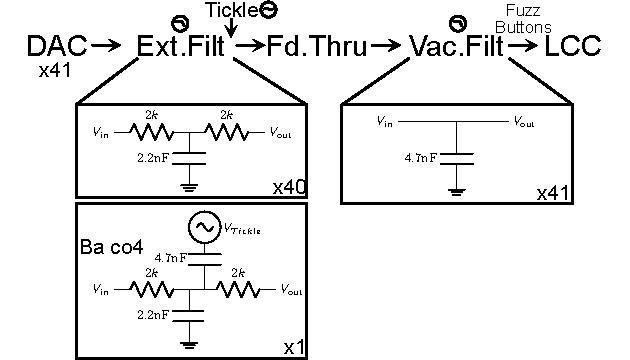
\includegraphics[width=0.6\linewidth]{figures/pdf_figure/ch2/dc_chain.pdf}
    \end{center}

    \noindent and embedded within the schematic~\ref{fig:apparatus}. Two
    multi-channel DACs, known as \emph{Fastino}, part of the \emph{Artiq Sinara} hardware
    ecosystem, provide the initial $41$ DC channels. 
    The Fastino outputs are filtered by a passive cascaded RC low pass filters with resistances, $R=2k$, and capacitances $C_1 = 2.2~\unit{\nano\farad}$ and $C_2 = 4.7~\unit{\nano\farad}$\footnote{For in-vacuum use. 1206 NPO 4.7nF 100V, SRT 1206A472JBCB} yielding a $-3$~dB ``cut-off'' frequency of $7.4~\unit{\kilo\hertz}$. The low pass filter circuit is shown in the above schematic, with the first stage on an external to vacuum PCB (Ext. Filt), and the 
    final shunt capacitor on an in-vacuum PCB (Vac. Filt)\footnote{Vacuum compatible PCB using Rogers RT6002. Filter boards were designed by Mariella Minder.} within close proximity of the trap chip to mitigate RF pickup on the DC lines. The feedthrough to the vacuum system has 51 pins\footnote{\emph{Allectra} 51-way Micro-D} with non-DC pins used to provide ground connections.
    On the external filter board, one channel, corresponding to electrode \textit{Ba co4}, has a capacitively coupled in AC signal. This originates from a DDS (\emph{Urukul}) and is used to resonantly excite the motional modes of the ion chain for characterisation and calibration purposes (see section~\ref{sec:Motional Mode Stability}).
    The in-vacuum PCB is connected to the trap chip via a custom PEEK interposer with embedded \emph{Fuzz buttons} vias\footnote{\emph{Custom Interconnects} Au/BeCu 0.025" diameter x 0.104" length Fuzz Button}.\\
    The ion is confined in the ``operation'' zone, seen in
    figure~\ref{fig:trap} $(c)$. The axial trapping is provided by electrodes
    \textit{Ba dc5} and \textit{Fr dc5}, where $Ba$ and $Fr$ correspond to the back and front plane of the trap respectively.
    The DAC can provide up to $10~\unit{\volt}$ to these electrodes to produce an axial frequency of $1.6~\unit{\mega\hertz}$.

\subsection{System Grounding}
% Main points:
    % Describe Fastino DAC and the available electrodes on the NPL trap
    % Quote values we use.
% Pre reqs:
    % NPL trap geometry
    % RF chain
    % DC voltages
    % Block diagram of the system
    % Vacuum system
    \todo{Thinking of removing this section.}
    Poor ground design (or no design at all).
    RF signal and return in vacuum may be important.
 
\section{Magnetic Field}
\label{sec:Magnetic Field}
% Main points:
    % Permanent magnets
    % MUMetal box
    Due to the fragility of
    the internal states of the ion (these are \textit{literally}
    state-of-the-art magnetic field sensors), we must take great care in
    isolating the ion from a noisy
    environment.
    We do not have access to magnetic field insensitive transitions in \ca , therefore uncontrolled Zeeman shifts of the internal atomic energy levels must be suppressed through enforcing a stable external magnetic field. This magnetic field stability is required for long spin
    coherence times (see section~\ref{sec:Coherence}), and for low error single-
    and two-qubit gates. A permanent magnet array of Samarium Cobalt\footnote{\emph{Bunting Magnets} E643SM and E644SM.},
    Sm$_2$Co$_{17}$, is used in a Helmholtz configuration to create a stable magnetic
    field of $\simeq 5~\unit{\gauss}$\footnote{Designed and constructed by Sophie Howarth.}. Samarium Cobalt was chosen for its low temperature
    coefficient of remenance, -0.03\%/K.\\
    The ion is shielded from unwanted external magnetic fields by a custom designed MuMetal enclosure\footnote{\emph{Magnetic Shields} custom
    design.}, with an internal dimension of $650\times 650\times 650~\unit{\milli\meter}$. The shielding consists of two layers of
    MuMetal shielding with internal shield thickness of $1.5\unit{\milli\meter}$ and external shield thickness of $2.0\unit{\milli\meter}$. The factory quoted
    shielding factor at the center of the box is
    $\times 546$ for DC fields. Spin coherence time comparisons with and without
    magnetic shielding are shown in
    section~\ref{sec:Coherence}.\\

\section{Vacuum System and Beam Geometry}
\label{sec:Vacuum System}
% Main points:
    % Technical drawing of beam geometries and magnetic field to ion chain.
    % In vacuum prisms
    % Materials and techniques used
    % Drawing of ion trap package with high NA lenses
        % High NA sandwich
    % Standing waves at the ion
% Pre reqs:
    % NPL trap
    % Why we have Dual high NA lenses
    % Magnetic field giving Zeeman shift


\begin{figure}
  \begin{center}
   \noindent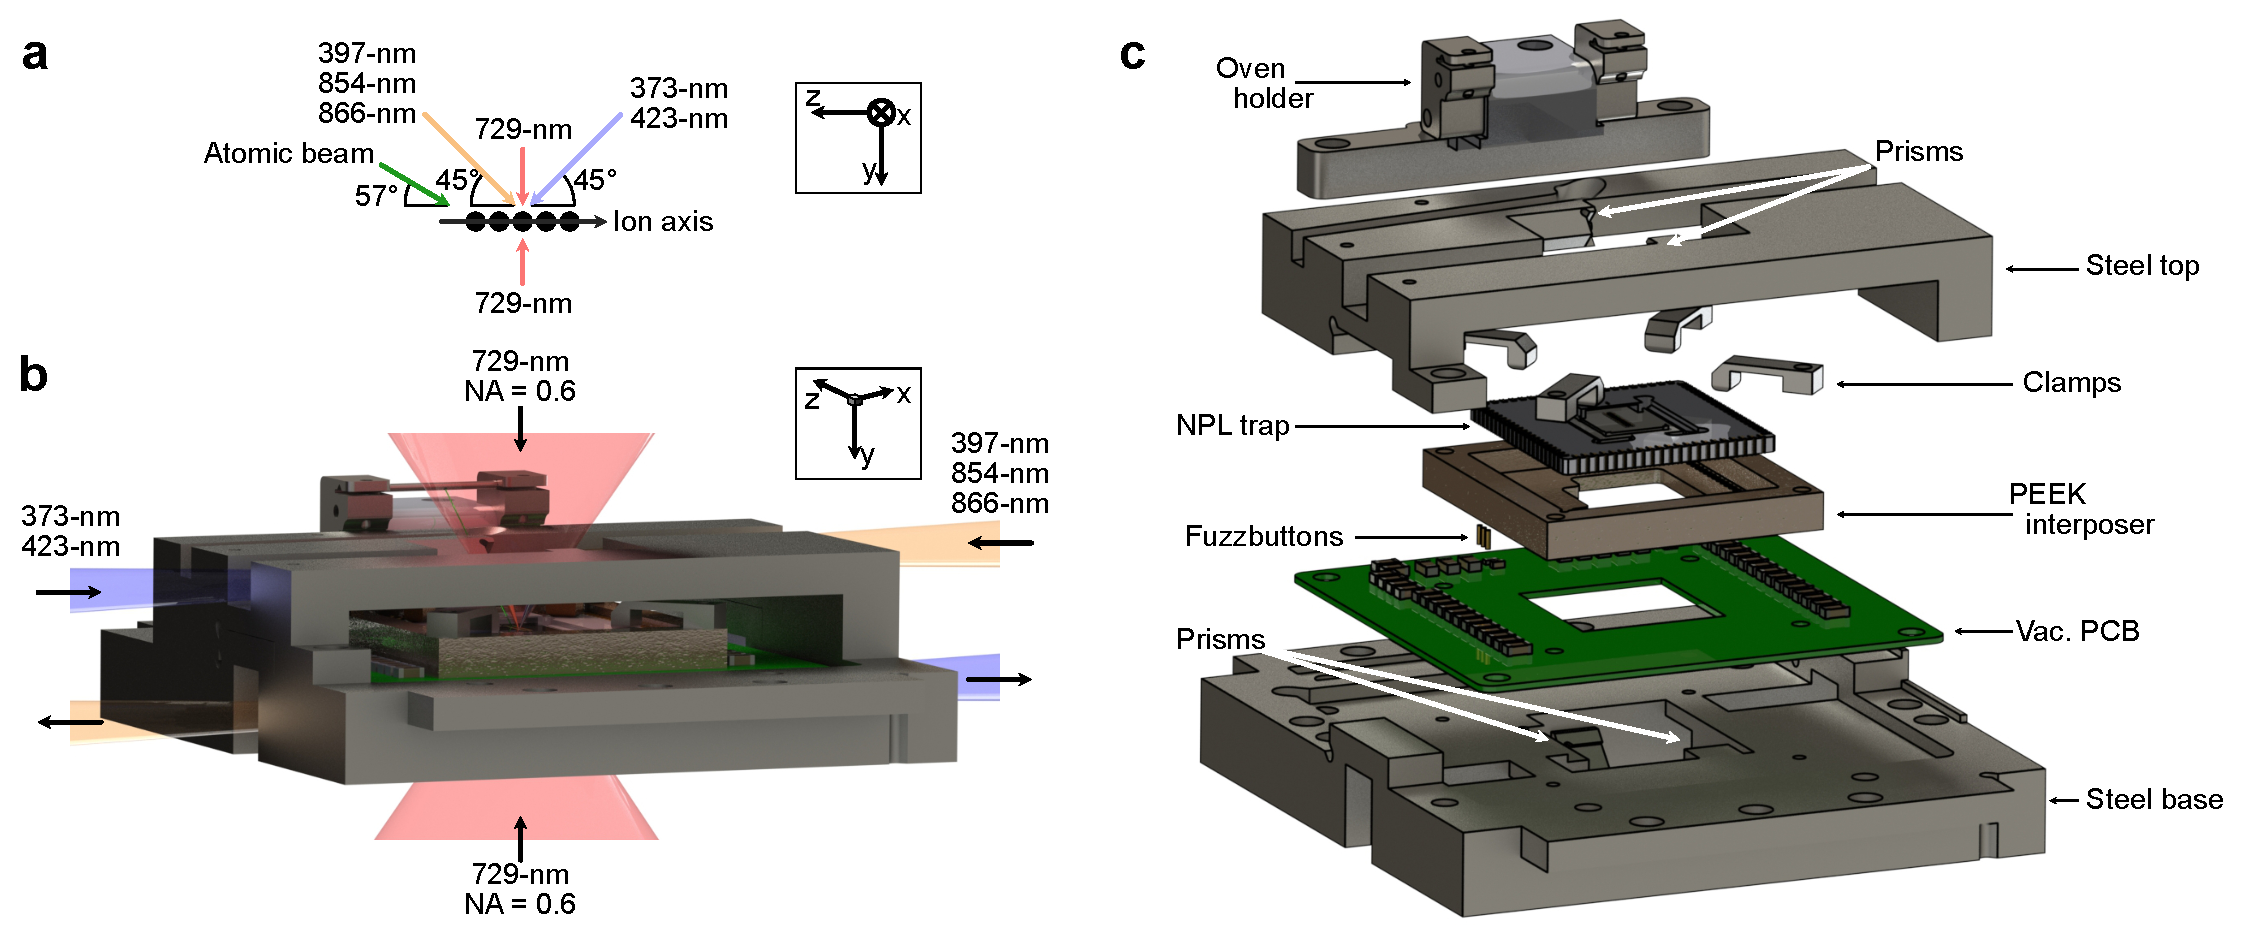
\includegraphics[width=\linewidth]{figures/pdf_figure/ch2/trap_package.pdf}
  \end{center}
  \caption{
    \textbf{a)} Laser and atomic beam geometries with respect to the ion chain.
    \textbf{b)} Compact trap housing with dual NA=0.6 access. The size of the high NA objectives restricts access for other beams, and so in-vacuum mirrors are used to redirect low-NA beams (373, 397, 423, 854, 866-nm) to the trap center.
    \textbf{c)} Exploded view of the trap housing with components labelled.
  }
  \label{fig:trap_package}
\end{figure}


\begin{figure}
  \begin{center}
   \noindent
\includegraphics[width=\linewidth]{figures/pdf_figure/ch2/HNA_package.pdf}
  \end{center}
  \caption{
    Cross section of the vacuum chamber and dual high NA objective sandwich. Lower right inset shows the vacuum chamber housed in the MuMetal enclosure, with dashed lines indicating the cross section region.
    Custom recessed CF-100 viewports are used to provide optical access for the high NA objectives (working distance $= 24.4~\unit{mm}$).
    }
  \label{fig:HNA}
\end{figure}

    Ultra High Vacuum (UHV) is required to prevent ion loss.
    However, UHV equipment is often bulky, and puts constraints on the access
    and visibility of the ion chain. Here, we describe the custom vacuum
    system, allowing for multiple beam access geometries including dual high numerical aperture (NA) objectives required for single addressed optical standing waves.  The vacuum system was
    designed by Sebastian Saner, Chris Ballance, and Mariella Minder, and constructed by
    Sebastian Saner, Fabian Pokorny, and myself.\\
    A residual pressure of $<10^{-11}$ mbar is desired. For this strict
    requirement, care must be taken in selecting in-vacuum materials, and 
    thorough cleaning and baking procedures must be followed. A summary of tactics that were
    useful in the construction of the vacuum system can be found
    in~\cite{birnbaum_ultra-high_nodate, wolf_cryogenic_2019}.\\
    The system consists of a 6" spherical-octagonal
    experimental chamber\footnote{Kimball MCF600-SphOct-F2C8} connected to a
    spherical chamber with ion pump\footnote{Agilent VacIon Plus 20 Pump}, ion
    gauge\footnote{Agilent UHV-24P Ion gauge} and Titanium sublimator pump
    (TSP)\footnote{Scanwel custom housing} attached. 
    After the final system bake, a He leak test was performed and 
    no external leaks were found. We do observe a gradual pressure increase that we suspect is either due
    to the in-vacuum optics, the optics epoxy adhesive\footnote{EPO-TEK
    353ND}, or the PCB solder. Regardless, the ion pump and TSP
    maintain UHV at the desired $<10^{-11}$~mbar (the TSP
    is fired every 4 weeks at 41~A for 60 seconds to provide a fresh Ti layer).\\
    Figure~\ref{fig:trap_package} $(a)$ shows the beam geometries with respect
    to the ion chain axis. The quadrupole 729-nm beam has high NA ($\mathrm{NA}=0.6$) access
    perpendicular to the ion chain axis, while 373-nm, 397-nm, 423-nm, 854-nm and 866-nm
    beams have low NA ($\mathrm{NA}<0.05$) access at an angle of $45^{\circ}$ to the ion chain axis.
    The atomic beam from the oven is at an angle of $\sim 57^{\circ}$ to the ion
    chain axis. As such, there is a doppler shift of the atomic beam with
    respect to the 423-nm photoionisation laser, which is accounted for in the
    set laser frequency (given $12^\circ$ angle between atomic and 423-nm
    beam, and 500~K mean temperature, expect $+126~\unit{\mega\hertz}$ frequency
    shift). Figure~\ref{fig:trap_package} $(b)$ shows the custom trap housing including NA=0.6 access for the 729-nm beams, and in-vacuum mirrors (prisms) to redirect the low NA beams to the trap center. The low NA beams enter the housing via one of the four beam access channels parallel to the trap chip plane, and are reflected through the trap slit. The exiting beam is reflected by a second mirror out of the housing to prevent scattered light incident on the ion chain.
    Figure~\ref{fig:trap_package} $(c)$ shows an exploded view of the trap housing with components labelled. The trap chip is interfaced to an in-vacuum PCB (described in section~\ref{sec:Trap DC Voltages}) via a custom PEEK interposer with embedded \emph{Fuzzbutton} vias (one for each DC and RF channel). The trap chip is held in place by 4 steel clamp arms, which attach to a steel base plate which provides mechanical stability and houses the lower in-vacuum prisms. A top steel plate houses the upper prisms. The tube oven is mounted on two steel clamps which are electrically isolated from the base plate by a PEEK spacer. The trap housing is fastened to the vacuum can by 4 steel arms attached to alternating side ports of the octagonal chamber~\footnote{Using \emph{Kimball Groove grabbers} P/N 53-482610}. Figure~\ref{fig:HNA} shows a cross section of the vacuum chamber and recessed dual high NA objectives. 
    Two recessed CF100 viewports\footnote{\emph{UK Atomic
    Energy Authority} P/N VPR100015} are required to bring the custom objectives\footnote{\emph{Photon Gear, inc.} Custom 18WD Atom Imager} to the designed working distance of 24.4~mm from the ion chain. 

\section{Imaging System}
\label{sec:Imaging System}
% Main points:
    % Describe the imaging system
    % Describe the camera and its properties
    % Describe the imaging optics and their properties
% Pre reqs:
    % High NA

\begin{figure}
  \begin{center}
   \noindent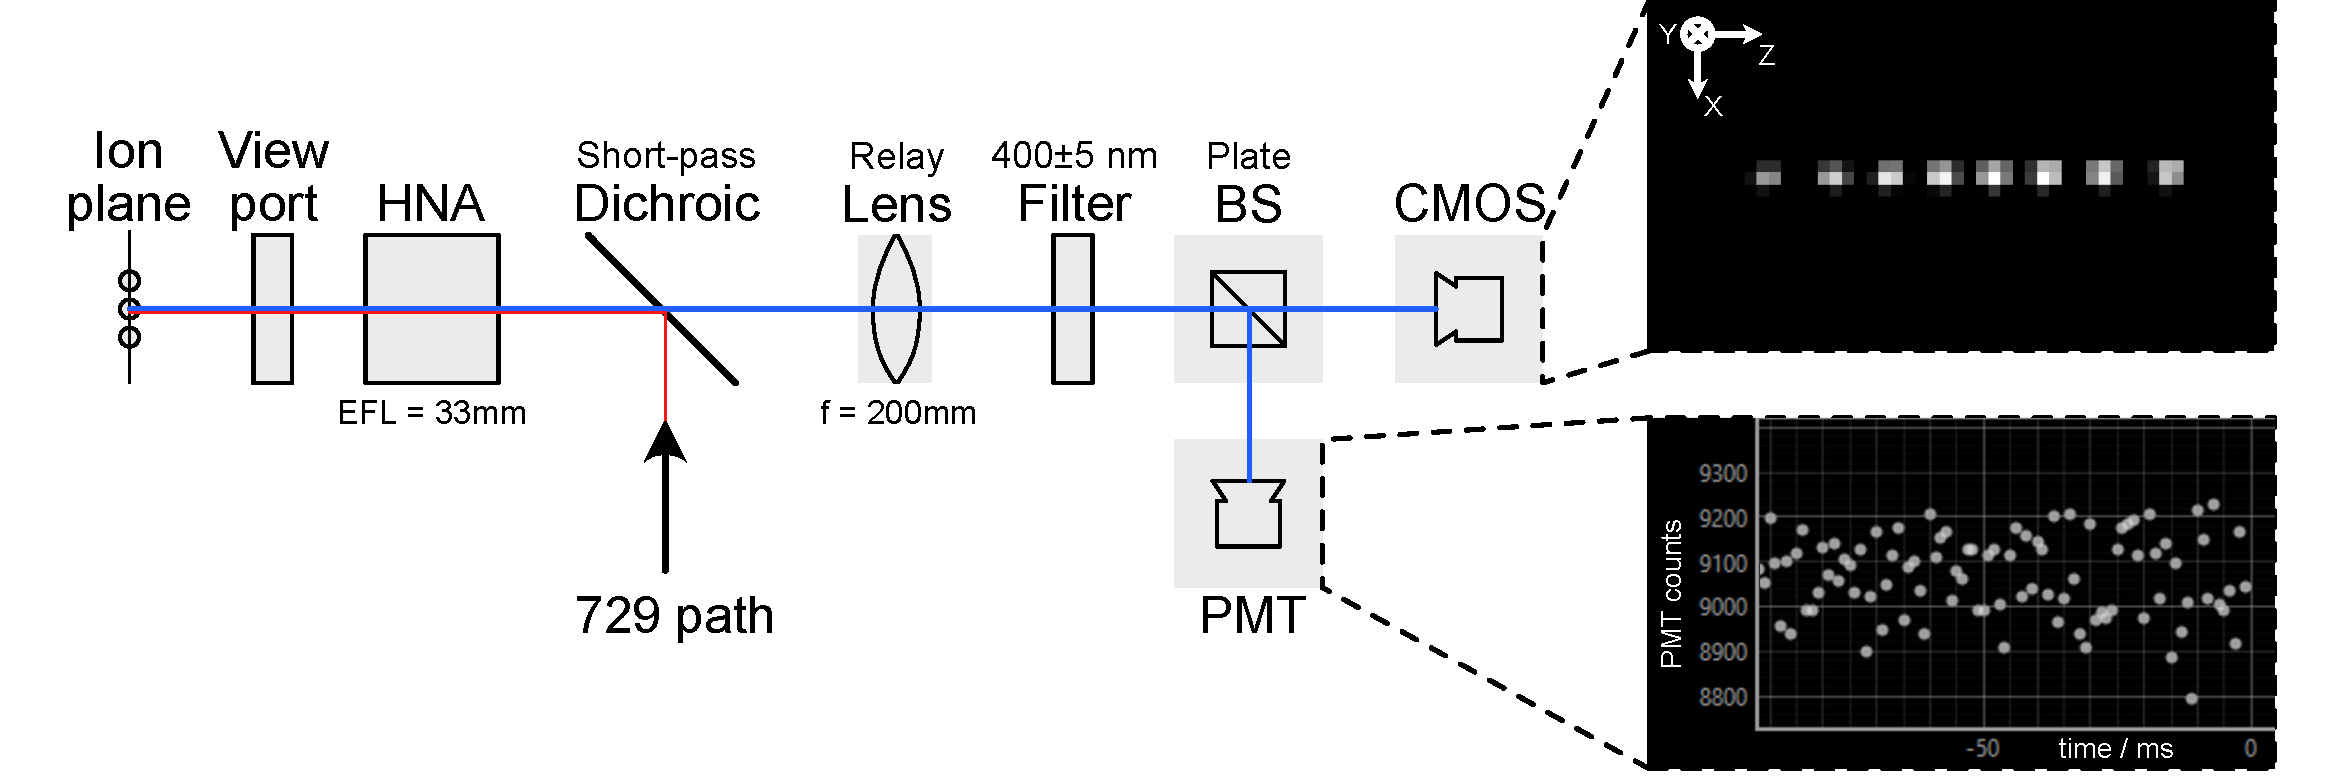
\includegraphics[width=0.9\linewidth]{figures/pdf_figure/ch2/readout.pdf}
  \end{center}
  \caption{Optical path for fluorescent imaging of the ions using both a CMOS camera and a Photon-multiplier tube. Insets on right hand side show typical signal for: spatial resolution of eight ions in a linear chain (top), time resolution of detected photons from the ion chain (bottom).
    }
  \label{fig:readout}
\end{figure}

    To image the ion chain, and readout the qubit states, fluorescent scatter of incident 397-nm light is collected. Here we briefly describe the imaging system, while section~\ref{sec:Measurement} describes the qubit readout procedure and fidelity. The imaging system is designed to provide high spatial resolution of the ion chain, while also providing a large field of view to accommodate long ion chains. The imaging system must also be compatible with the high NA objectives used for single addressed optical standing waves.
    Figure~\ref{fig:readout} shows the optical path schematic of the imaging system, with both a
    a high quantum-efficiency ($\simeq 70\%$ at $397~\unit{\nano\meter}$) 
    CMOS camera\footnote{\emph{Hamamatsu Orca-Fusion
    BT} C15440-20UP} for spatially selective qubit readout on a multi-ion chain, and 
    a photon multiplier tube (PMT)\footnote{\emph{Hamamatsu} Photon counting head H10682-210}, for experiments requiring time resolved photon counting (e.g. micromotion compensation, section~\ref{sec:Micromotion}).
    Typical signals of both devices can be seen in right panels of figure~\ref{fig:readout}. 
    The optical path consists of a high numerical aperture objective\footnote{\emph{Photon Gear, inc.} Custom 18WD Atom Imager} (effective focal length, $f=33~\unit{\milli\meter}$), $\mathrm{NA}=0.6$, a dichroic mirror\footnote{\todo{\emph{Thorlabs} TODO}} (transmission: $397~\unit{\nano\meter}$; reflection: $729~\unit{\nano\meter}$), a relay lens\footnote{\emph{Thorlabs} Achromat Doublet, ACT508-200-A-ML} ($f=200~\unit{\milli\meter}$), a $90:10$ plate beamsplitter\footnote{\todo{\emph{Thorlabs} TODO}}, and the camera and PMT. \\
    The objective lens is custom designed to compensate for aberrations due to the recessed vacuum viewport, however, due to the large NA, accurate alignment of all degrees of freedom of the objective is critical. As such, the NA is attached to a 5-axis alignment stage\footnote{\emph{Newport ULTRAlign} M-562-XYZ, M-36, SM-13}, with z-axis focus controlled by a piezo micrometer\footnote{\emph{Newport CONEX-TRA12CC}} for fine adjustment of the ion focus with the MuMetal box closed (requires $<\unit{\micro\meter}$ precision).\\
    Given the chosen lens focal lengths, we expect a magnification of $\times 6$ from the ion plane to the imaging plane. With an expected ion separation of $5~\unit{\micro\meter}$, and the camera pixel pitch of $6.5~\unit{\micro\meter}$, we expect around 4.5 pixels between ions, which, if the system is well aligned, is more than sufficient for low cross-talk spatial readout of qubits.
    % Could add alignment tactics
    % Could add how this can be improved?
    
\section{Ca$^+$ Laser Systems}	
\label{sec:Laser systems}
% Main points:
    % State which lasers we need access to
    % Calcium level structure 
    % Beam paths
    % What frequency control do we need on each? PDH lock, AOM etc.
    % Table of all AOMs and offset frequencies
    % Table of laser powers in mW and with aimed saturation intensities for doppler idle, cooling, readout, and laser linewidths.
    % Intesity stabilisation using SUServo
% Pre reqs:
    % Calcium level structure
    % 5 G field

    Singly-charged group 2 elements are popular in ion trap
    experiments due to their single outer electron resulting in Hydrogen-like
    energy levels. In this thesis we use \ca.\\
    \ca has
    no nuclear spin giving the
    (relatively) simple level structure shown in figure~\ref{fig:ion} with the relevant laser transitions used in our apparatus are indicated. Details on the ion choice, and utility of the lasers is given in section~\ref{sec:Transitions}, here we only describe the hardware and feedback control to provide this stabilised light.\\
    The relevant wavelengths are the following:
    The qubit is defined by the quadrupole transition at 729-nm. Access to other excited levels, outside of our defined two level system, are crucial for ion trap quantum logic to enable qubit readout via state selective fluorescence (397-nm, and 866-nm transitions), and state preparation via optical pumping (866-nm, and 854-nm transitions). Access to two additional transitions in neutral calcium for isotope selective ionisation, 423-nm and 373-nm, are also required~\cite{lucas_isotope-selective_2004}.\\
    This section begins with a description of laser frequency and power stabilisation techniques common to multiple laser systems used in this thesis. Following this, the specific systems are described, starting with 
    the diode lasers, which drive all but the 729-nm transition. Subsequently, the Ti:Sapph 729-nm source is discussed. Finally, the global and single addressed beam arrangements for the 729-nm system are described.\\

\subsection{Frequency Stabilisation}
    % PDH scheme
    \begin{figure}
    \begin{center}
    \noindent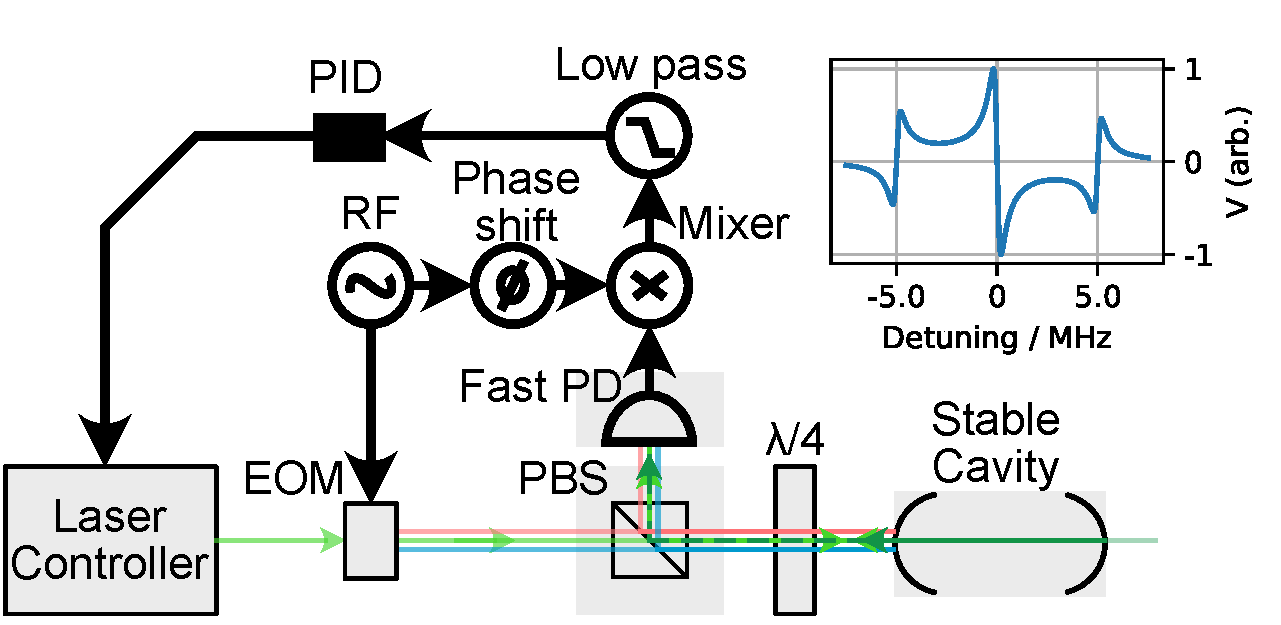
\includegraphics[width=0.7\linewidth]{figures/pdf_figure/ch2/pdh.pdf}
    \end{center}
    \caption{PDH optical and control schematic. Green optical path represents the carrier frequency, blue and orange lines represent the upper and lower sidebands respectively, generated by an EOM. The reflected light is directed onto a fast photodiode, and the signal is demodulated with the same oscillator signal used to drive the EOM, but delayed by some chosen phase. The signal is finally low pass filtered to recover the error signal, an example of which is seen in the upper right panel for a finesse $F\sim 4000$, a free spectral range of $FSR = 1.5~\unit{\giga\hertz}$, and a modulation frequency of $f_{mod} = 5~\unit{\mega\hertz}$. 
        }
    \label{fig:PDH}
    \end{figure}
    All lasers exhibit frequency noise due to unavoidable environmental coupling
    (e.g. temperature fluctuations, and acoustics), and to instabilities in
    control signals (e.g. voltage and current controls). For the lasers
    corresponding to dipole transitions used in this thesis, we are relatively
    lenient and require slow frequency excursions of $<1~\unit{\mega\hertz}$
    with respect to the qubit transition, and laser linewidths less than the
    natural linewidth of the dipole transitions, which are often multiple MHz.
    However, for the quadrupole transition at 729-nm, we require significantly
    more stringent frequency stability, with laser linewidths of
    $<100~\unit{\hertz}$, and negligible phase modulation of the laser light
    over a few MHz of the qubit transition to ensure spectator transitions are
    not excited during qubit operations. 
    Although the order of magnitude of the
    required frequency stability is different for the dipole and quadrupole
    transitions, the concepts and techniques used to achieve this stability are similar. Generally, a closed loop consisting of measurement of the optical frequency of the laser and feedback to the laser control is required. In this work, stable external optical cavities are used for referencing the laser frequency. Specifically, 
    we use the Pound-Drever-Hall (PDH) 
    techniques to generate the error signal for the feedback loop. The PDH technique is well described in the literature~\cite{drever_laser_1983, oswald_characterization_2022, black_introduction_2001}, and so here we only give a brief overview of the technique to contextualise the required hardware introduced in the following sections.\\
    The conceptual goal of the PDH technique is to measure the frequency difference between the laser and a resonant frequency of a stable optical cavity to generate an error signal, preferably linear over typical frequency excursions (while \emph{locked}). This error signal can then be modified by some controller (typically PID), to directly infer how to tune the laser controls to minimise this error signal, often termed \emph{locking} the laser to the cavity. Further, the error signal should be insensitive to amplitude noise on the laser light, to avoid amplitude to frequency noise conversion due to the feedback loop (in contrast, side-of-fringe stabilisation is sensitive to amplitude drifts).\\ Practically this scheme consists of phase modulation of the incident laser light, here by electro-optical modulators (EOMs), to generate sidebands, which are used as phase references to compare the phase of the incoming laser field to that of the phase of the field inside the cavity. Figure~\ref{fig:PDH} shows a schematic of the PDH scheme, highlighting the beam paths and closed loop. The phase modulated light is directed onto the cavity, with the total return signal being some combination of the reflected sidebands, carrier, and the cavity leakage field, with the latter providing the phase of the electric field inside the cavity. The reflected light is directed onto a fast photodetector, and the signal is demodulated with the same oscillator signal used to drive the EOM, but delayed by some chosen phase. The resulting signal is low pass filtered to remove high frequency components, yielding the final error signal, an example of which is seen in the upper right panel of Figure~\ref{fig:PDH}. The central region is anti-symmetric and linear, centered on the desired lock point. Using a tuned controller for feedback to the laser controller, this provides a stable lock of the laser to the cavity.\\
    As the cavity is used as a frequency reference, both a high finesse and stable optical lengths are desirable. The gradient of the PDH error signal is proportioanl to finesse, leading to increased signal to noise with higher finesse (see Ref.~\cite{oswald_characterization_2022} for more details). Optical length deviations are minimised through mounting the cavity in a vacuum chamber, and taking care in isolating it from temperature fluctuations and vibrations.\\
    Particular details of the PDH hardware and control loops are given in the following sections for each laser system. \\

\subsection{Intensity Stabilisation}
\label{sec:Intensity Stabilisation}
    The light-matter interactions considered in this thesis are all proportional
    either to intensity or amplitude of the optical electric field at the ion's
    position. Intensity fluctuations over time therefore lead to fluctuations in the interaction strength, which are detrimental to the fidelity of quantum operations. 
    Intensity noise originates either from total beam power
    fluctuations, or due to beam pointing drift with respect to the ion
    position. The former is mitigated through a closed feedback loop between a
    pick-off photodiode signal before the ion monitoring the optical power, and
    the drive RF amplitude of an upstream AOM. 
    For all beams, this optical pick off is one of the last elements before the beam enters the vacuum system to reduce the impact of lossy elements between the stabilise point and the ion position.
    The low-noise photodiodes used were designed by David
    Nadlinger (\emph{QLNPD}), and the feedback system controller, known as \emph{SUServo}, was written by
    Peter Drmota.\\
    Beam pointing drifts are mitigated through careful mechanical design of the optical paths for passive stability, and through automated intermittant beam pointing calibrations using the ion as a sensor (see section~\ref{sec:Beam Pointing Calibration}).\\
    
\begin{figure}
  \begin{center}
   \noindent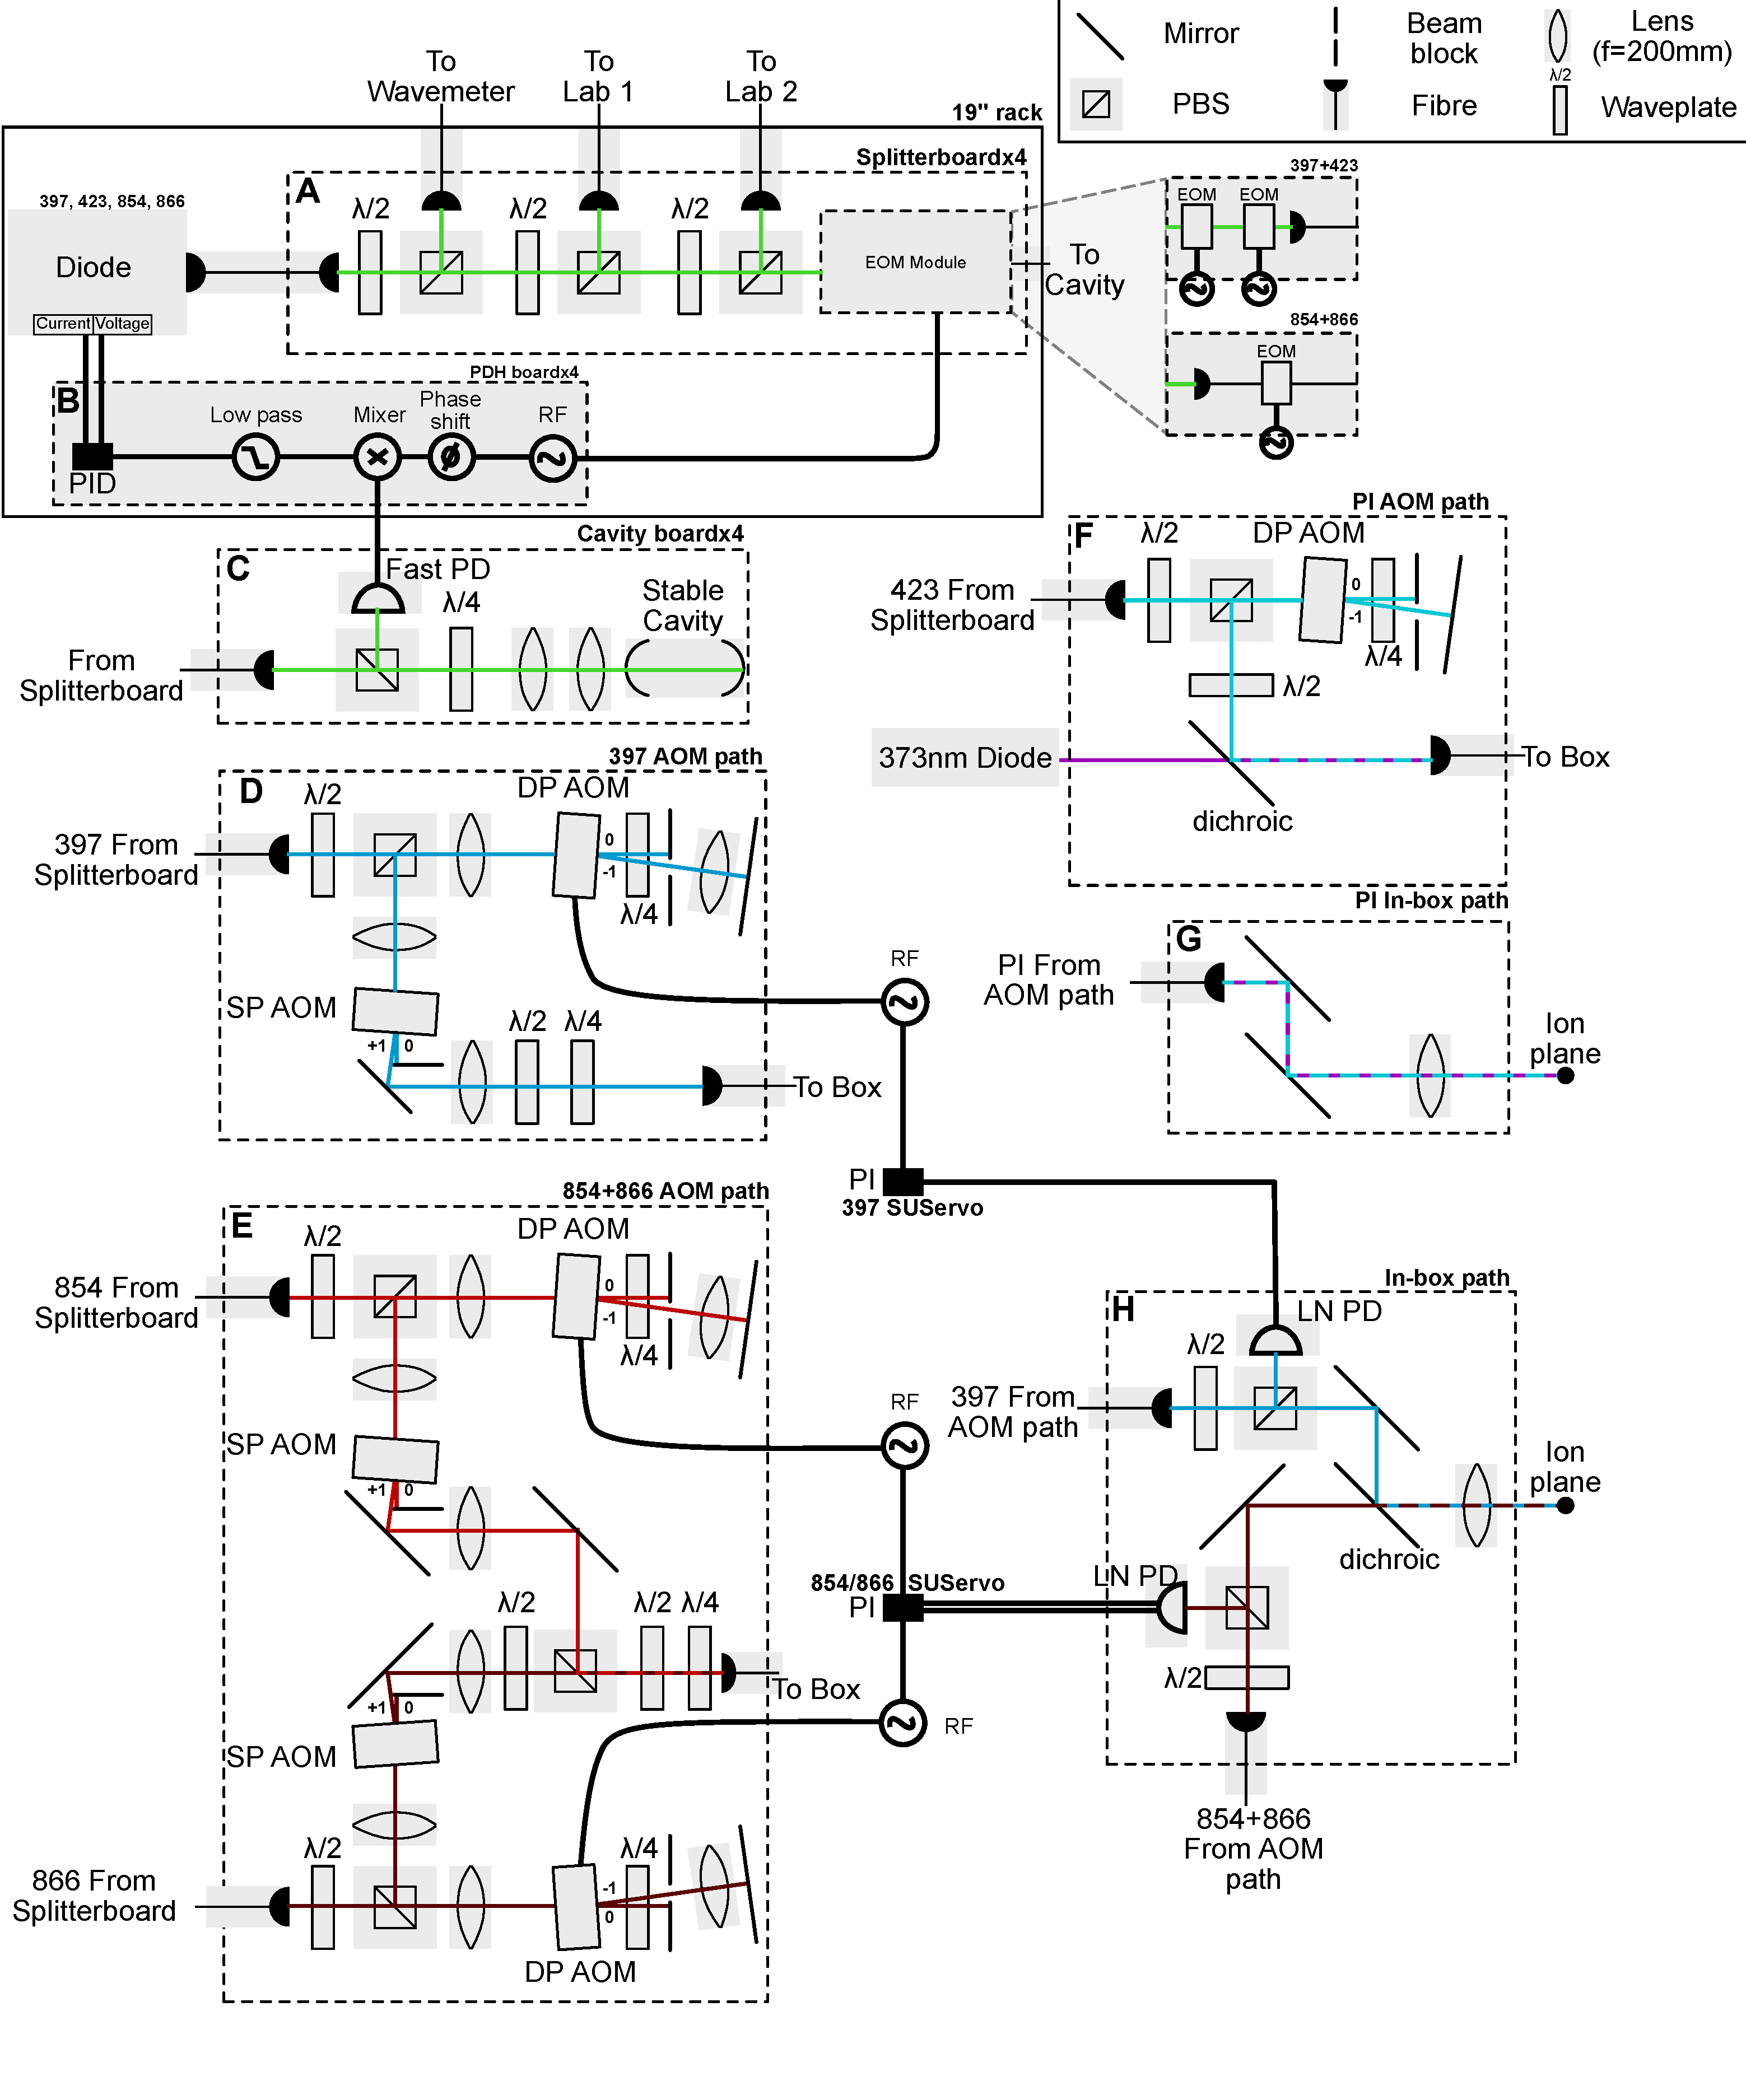
\includegraphics[width=\linewidth]{figures/pdf_figure/ch2/diode_paths.pdf}
  \end{center}
  \caption{
    All beam paths for diode laser systems. Dotted boxes resemble modular optical paths with fibre and control lines in and out only. Frequency and optical power control loops are included.
    }
  \label{fig:diode_paths}
\end{figure}

\subsection{Diode Lasers}
\label{sec:Diode Lasers}
% Four bore locking cavity
% Beam paths? AOM DP and SP?which are frequency stabilised to a reference cavity\footnote{\emph{Stable Laser Systems} SLS-6010 4-Bore Cylindrical Cavity} via Pound-Drever-Hall (PDH) locking. 
    %\mccorrect{XXX should quote finesse and FSR values here.}
    For transitions 397-nm, 854-nm, and 866-nm, we require light that is frequency stable
    to $<1~\unit{\mega\hertz}$ level, well below the natural line widths of the
    dipole transitions, and power stable to $<1~\unit{\micro\watt}$. 
    All beam paths and relevant control loops for the diode laser systems are
    shown in figure~\ref{fig:diode_paths}. The laser diode
    heads\footnote{\emph{Toptica} diodes. 854/866: MDL DL pro; 397: MDL DL pro
    HP; 423: DL pro}, controllers\footnote{\emph{Toptica} DLC Pro with PDH
    boards}, and splitterboards\footnote{Designed by \emph{OITG Cavities} group}
    (fig~\ref{fig:diode_paths} (a)) are housed in a single 19" rack. The
    splitterboard distributes the light between two ion-trap experiments, the
    PDH lock cavity (fig~\ref{fig:diode_paths} (c)), and a diagnostic wavemeter
    for checking wavelength and lock status\footnote{\emph{HighFinesse} WS7}.
    The splitterboard also houses an Electro-optic modulator (EOM) module for
    applying both offset and PDH sidebands for an offset PDH lock. The offset sidebands may be arbitarily set (within the $\unit{\giga\hertz}$ range of the EOM) to provide a continuous choice of laser lock frequencies between cavity modes, rather than maintaining a fixed offset between the laser output frequency and the discrete cavity mode frequencies. For 397-nm
    and 423-nm, resonant free space EOMs\footnote{\emph{Qubig} PM7-VIS-25 and PM9-VIS-2.25}
    are used, for 854-nm and 866-nm broadband fibre EOMs\footnote{\emph{EOSPACE} PM-0s5-05-PFA-PFA-850} are used
    for convenience. The path on the reference cavity board
    (fig~\ref{fig:diode_paths} (c)) consists of a four-bore reference
    cavity\footnote{\emph{Stable Laser Systems} SLS-6010-1-4bore} under vacuum and
    temperature control, two lens for matching the collimated input beam to the
    cavity mode, and a beamsplitter and $\lambda/4$ waveplate for directing the
    reflected cavity light to a fast photodiode\footnote{\emph{Thorlabs} PDA10A2}.
    The beatnote due to the carrier and PDH sidebands are mixed down and
    low-passed by the \emph{Toptica} PDH module to produce the signature
    antisymmetric PDH trace. Gains for PID controllers of both the diode current
    and voltage are set to stabilise the optical frequency.\\
    The light from
    the ``laser'' laboratory is carried to the ``trap" laboratory using 16~m
    polarisation maintaining fibres\footnote{\todo{\emph{Schafter-Kirchoff} ...}}. In
    the ``trap'' laboratory we use AOMs in a double pass configuration for both
    frequency shifting and power stabilising the light
    (fig~\ref{fig:diode_paths} (d) and (e)). \\
    As space inside the MuMetal enclosure is constrained, it is advantageous to
    couple multiple beams in a single fibre before the enclosure.
    The second stage photo-ionisation light, at 373-nm\footnote{\emph{Toptica} iBEAM-SMART-375-S.},
    is combined with the 423-nm beam by a dichroic
    (fig~\ref{fig:diode_paths} (f)) before being coupled to a 16~m fibre that
    takes the light directly into the MuMetal enclosure. The respective refractive indices of fused silica  for 373-nm and 423-nm differ to the extent that the two beams were separated by more than one waist at the ion plane after initial rough alignment. To ensure the two beams overlap at the ion plane, care was taken for the beam propagation to be perpendicular to both the lens and vacuum viewport window, and a parabolic mirror outcoupler\footnote{\emph{Thorlabs} RC02APC-F01} (rather than a lens) was used inside the MuMetal box.\\
    The 854-nm and 866-nm light is combined after
    their respective double and single pass AOMs, and coupled into a 3~m PM\footnote{\todo{\emph{SK} ...}}
    fibre carrying the light into the enclosure.\\
    Light from both the PI and the 397/854/866-nm paths are directed onto the
    ions via the in-vacuum prisms, discussed in section~\ref{sec:Vacuum System}.
    The final mirrors prior to the vacuum system are
    motorised\footnote{\emph{Newport Picomotor} piezo mirror mount P/N 8821}, so that beam alignment to the ions
    can be optimised when the MuMetal enclosure is closed. Practically we find
    that these beams rarely need to be realigned (few months), unless there is a
    significant ambient temperature change of a few degrees.\\


\subsection{Narrow Linewidth 729 Laser}
\label{sec:Narrow Linewidth 729 Laser} 
% Main points:
    % What equipment does the 729 consist of.
    % Solstis cavity
    % Beam path and control loops (PDH, FNC)
    % Frequency shifting, pulse carving via urukul
    % Amplitude stabilisation with SUServo
% Pre reqs:
    % Calcium level structure
    Lasers are a key tool for creating the highly localised, strong electric
    field amplitudes and gradients needed to drive both carrier and sideband
    transitions of the trapped ion.\\
    As shown in Figure~\ref{fig:ion}, 
    two sublevels within the 4S\textsubscript{1/2} to 3D\textsubscript{5/2}
    manifolds define the qubit. This is an electric quadrupole transition as
    $\Delta l = 2$.  For the Calcium ion this transition is at 729-nm, and so 
    a near resonance 729-nm laser is used to implement single- and multi-qubit gates
    (sections~\ref{sec:Single Qubit Gates} and~\ref{sec:Two-Qubit
    Entangling Gates}). This transition is also used after Doppler cooling for
    resolved sideband cooling to prepare the motional mode close to its ground
    state (as discussed in section~\ref{sec:Cooling}).
    This transition is narrow linewidth due the the long lived
    3D\textsubscript{5/2} level, and so, for power efficiency, a
    narrow linewidth laser must be used. For the ``fast entangling gates'' use-case, high intensity electric-fields are required at the ion to drive sideband
    transitions, this will be discussed further in the single-addressing and
    two-qubit gate sections, but here it is sufficient to say we require >100 mW
    of light at the ion plane.  Here we describe the 729-nm system 
    consisting of a Ti:Sapph laser system pumped by an Nd:YAG 532-nm laser.\\
    An \emph{M2 Solstis} Ti:Sapph is pumped via 18~W of 532-nm light
    from a \emph{Coherent Verdi-V} system to produce around 5~W of
    729-nm light.  The Ti:Sapph is engineered to operate with a stable $<50$~kHz
    linewidth. Ti:Sapph crystals have broadband gain profiles which
    make them amenable in research environments to create frequency tunable
    laser systems. They also often have lower intrinsic phase noise than diode lasers at the same wavelength, which is favourable for our application.
    For single mode operation, the \emph{Solstis} employs multiple intracavity frequency selective
    elements which consist of (in order of coarse frequency selectivity), a
    birefringent filter, a tunable Fabry-P\'erot etalon, and the surrounding
    bow-tie cavity. To lock the tunable etalon to one longitudinal cavity mode, an actively stabilised ``dither'' phase-lock loop is used. This dither consists of periodically varying
    the etalon spacing with a frequency of around 20~kHz. 
    This dither frequency direclty phase modulates the light, which leads to the creation of
    sidebands which can interact with the ion causing 
    errors in gates. This dither frequency (and harmonics of it), can be observed 
    via composite pulse experiments on the ion, and are discussed in section~\ref{sec:Coherence}.\\
    \begin{figure}
    \begin{center}
    \noindent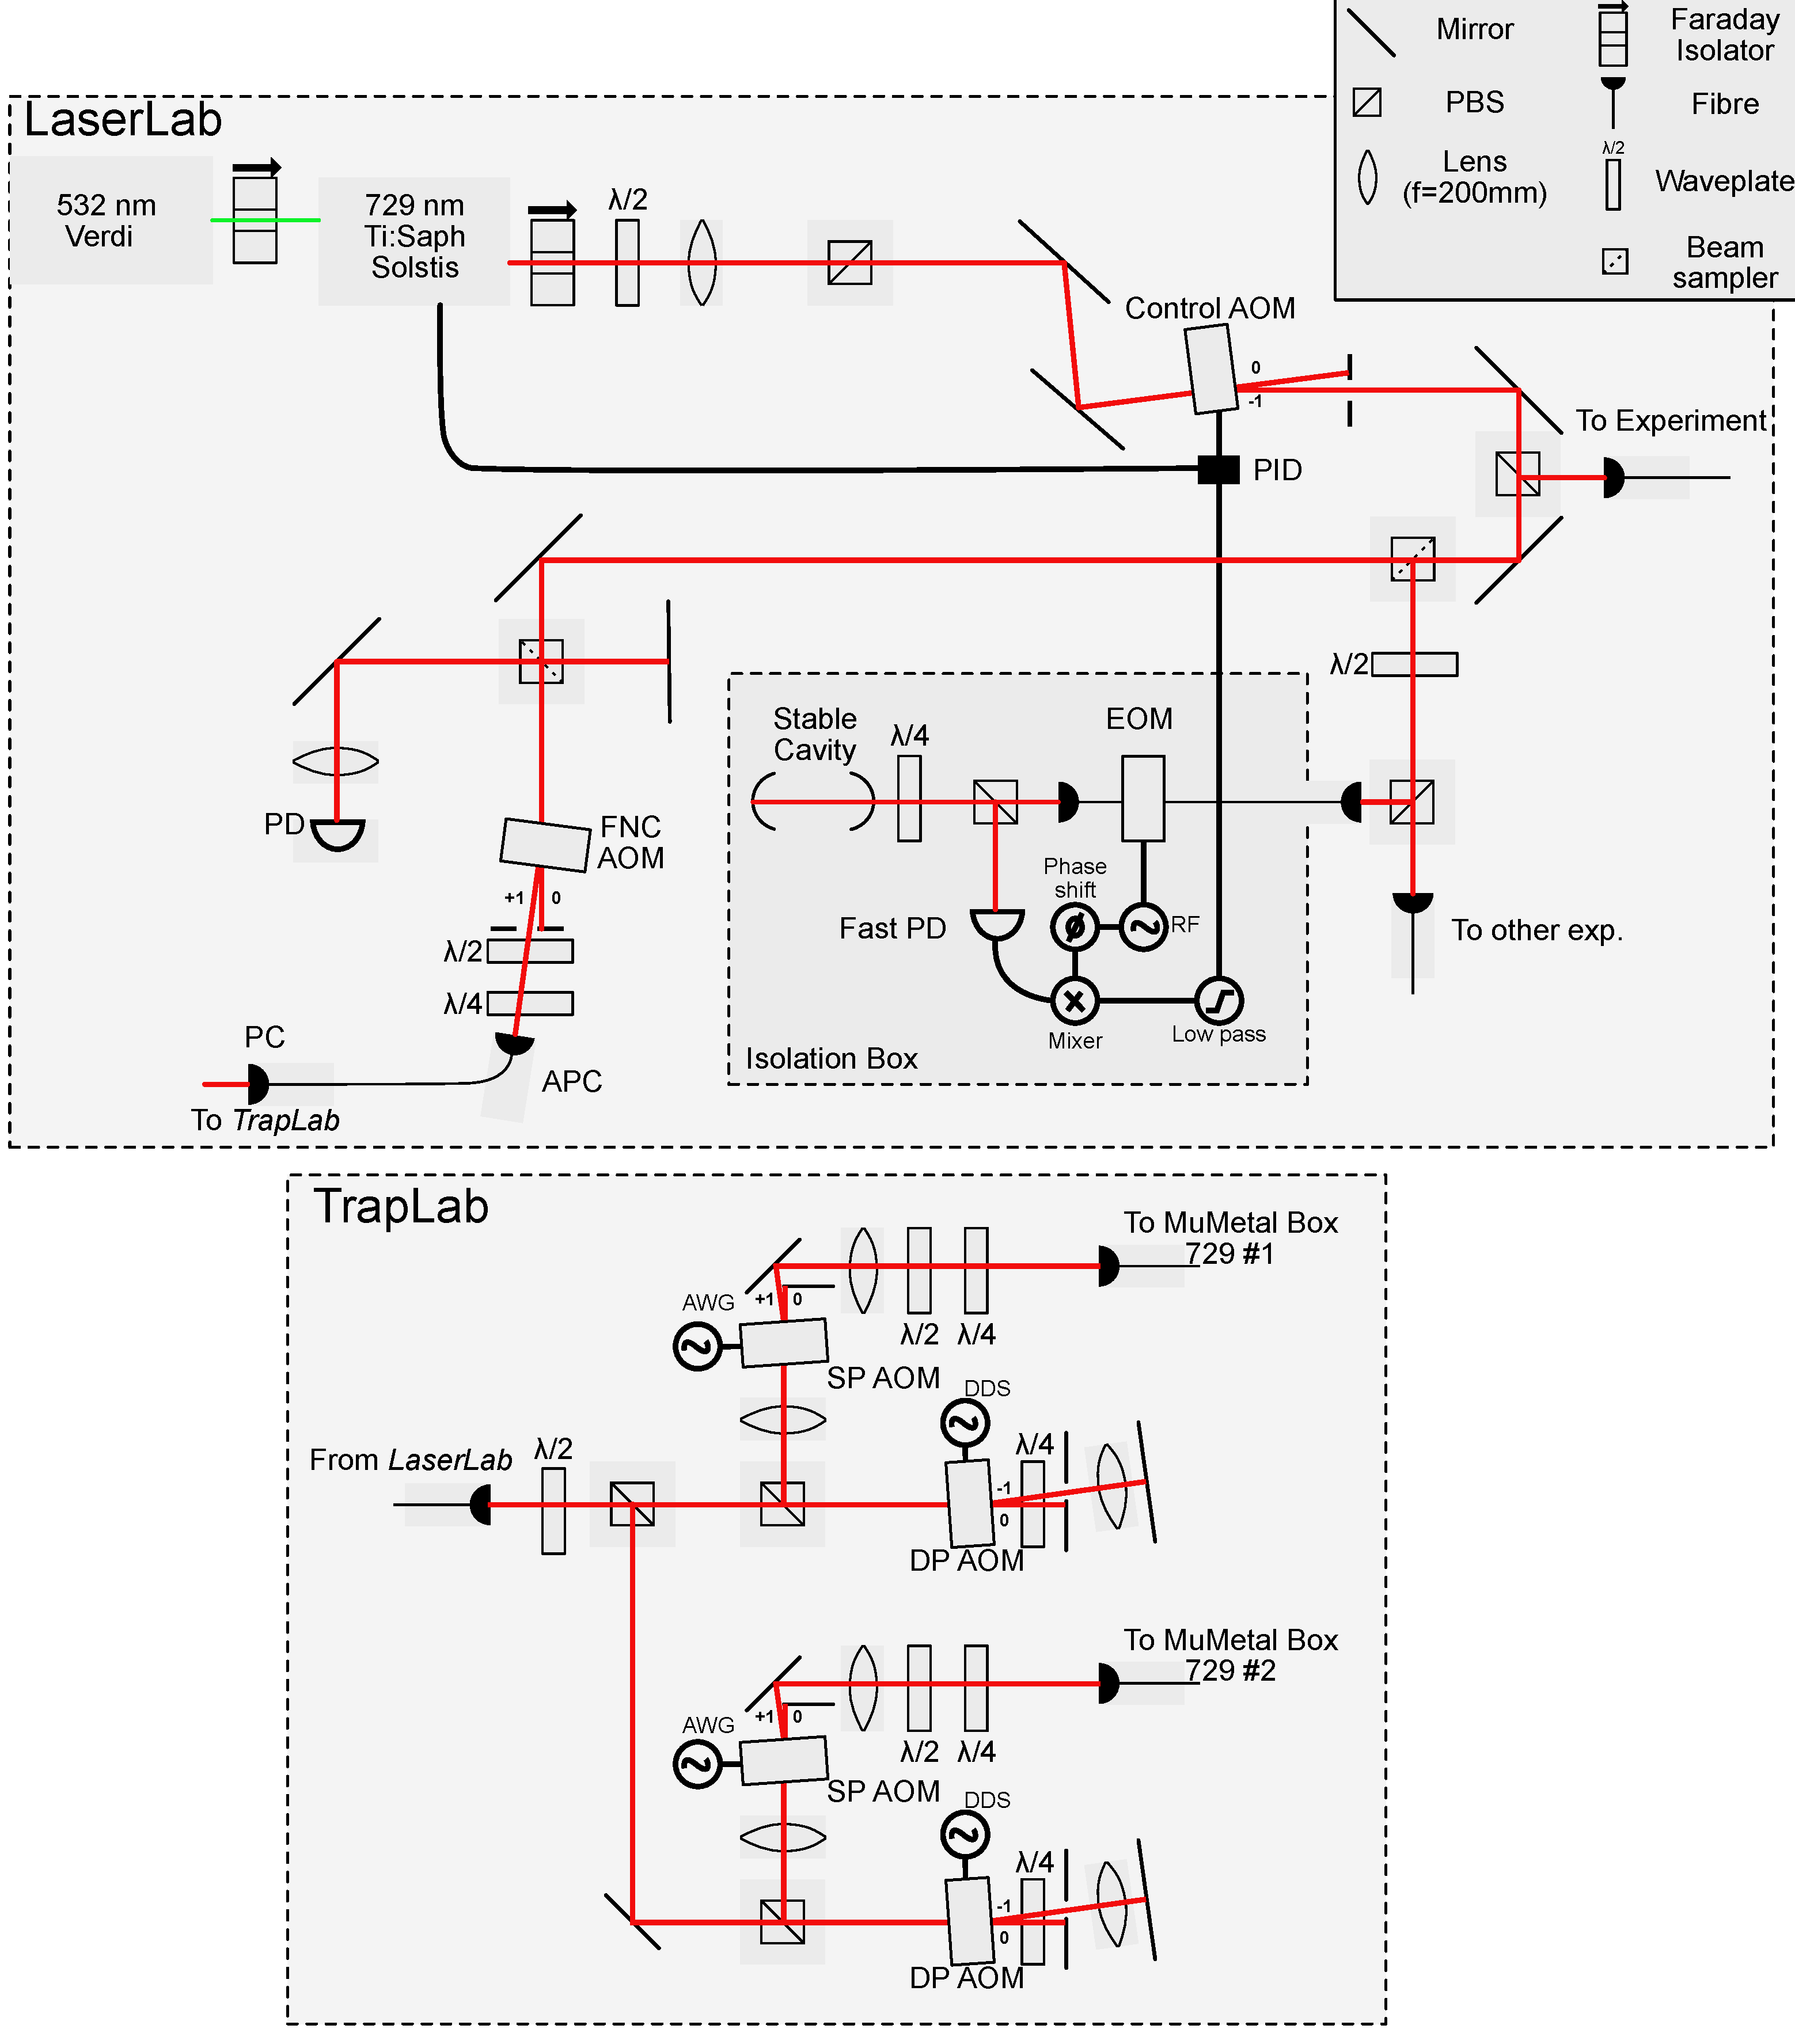
\includegraphics[width=\linewidth]{figures/pdf_figure/ch2/729_path.pdf}
    \end{center}
    \caption{The 729-nm system. A Ti:Sapph laser tuned to 729-nm is
        pumped by a 532-nm source. Light is picked off at the first beam
        sampler to stabilise by PDH locking to a cavity. Light is distributed to two experiments, with the \emph{FastGates} line including a fibre noise cancellation system.}
    \label{fig:729}
    \end{figure}
    \begin{figure}
        \begin{center}
        \noindent
\includegraphics[width=0.75\linewidth]{
            figures/pdf_figure/cavity_drift.pdf
            }
        \end{center}
        \caption{
            Cavity drift over 125 days measured by reference to the ion transition. The laser offset here is with respect to running all 729-nm AOMs at their central frequencies. Outliers are due to bad fits of the ion transition frequency, not due to changes in the cavity resonance.
            }
        \label{fig:Cavity Drift}
    \end{figure}
    Referencing the \emph{Solstis} output with an external cavity and using PDH feedback can greatly suppress phase noise. Here an ulta high finesse cavity\footnote{\emph{Stable Laser Systems} P/N 6020-4} is used, with a schematic of the 729-nm system 
    shown in Figure~\ref{fig:729}.  
    As opposed to the simpler controller implemented for the diode lasers, the 729-nm uses a cascaded PID lock with a fast feedback loop to the AOM situated after the Solstis, and an intermediate and slow feedback loop to piezos controlling the Solstis cavity length.
    % Give params here and topology of the cascaded PID loops.
    With this system, a linewidth of $<<1$~kHz for the 729-nm light is expected. 
    The electronics for this control loop are
    provided by \emph{Stable Laser Systems} in the form of their \emph{FPGA Servo}
    lock box. For an effective PDH lock, both short and long term
    stability of the reference cavity is required. To ensure the cavity is insensitive to
    the environment, it is made of an ultra low expansion material, and mechanically isolated from the environment by an acoustic dampening enclosure and a vibration isolation platform. The cavity is housed in a vacuum system to prevent refractive index fluctuations due to air, and to further reduce thermal coupling to the environment. 
    The cavity is temperature stabilised at the zero crossing temperature of
    $30.6^\circ$C. Long term cavity drifts of 309(1) Hz/hr are measured over
    125 days, seen in figure~\ref{fig:Cavity Drift}. This measurement uses the ion as a
    frequency reference to probe the cavity frequency, with details given in section~\ref{sec:Magnetic Field and Laser Offset}.\\
    Figure~\ref{fig:729} displays the other beam paths for our 729-nm system.
    Some light is picked off and sent to a wavemeter to continuously monitor the
    frequency. However, the majority is coupled to two output fibres for our
    experiment and another within the group. The 729-nm light is transported from
    a dedicated laser lab to a the trap apparatus lab by a 10~m
    single mode polarization maintaining fibre\footnote{\todo{\emph{SK} ...}}.  The fibre
    introduces phase noise due to mechanical and thermal pertubations along the 10~m
    length. To remove this introduced noise, passive stabilisation in
    the form of thick foam tubing along the fibre length, as well as active
    stabilisation by a fibre-noise-cancellation (FNC) technique~\cite{ma_delivering_1994}, is used\footnote{FNC control consists of \emph{Sinara Stabilizer} and \emph{Pounder}
    mezzanine board with PID software 
    developed by Ayush Agrawal.}. The efficacy of the FNC system is characterised in section~\ref{sec:Coherence} by measuring the spin coherence time of the ion.\\


\subsection{Single Addressing System}
\label{sec:Single Addressing System}
    \begin{figure}
        \begin{center}
        \noindent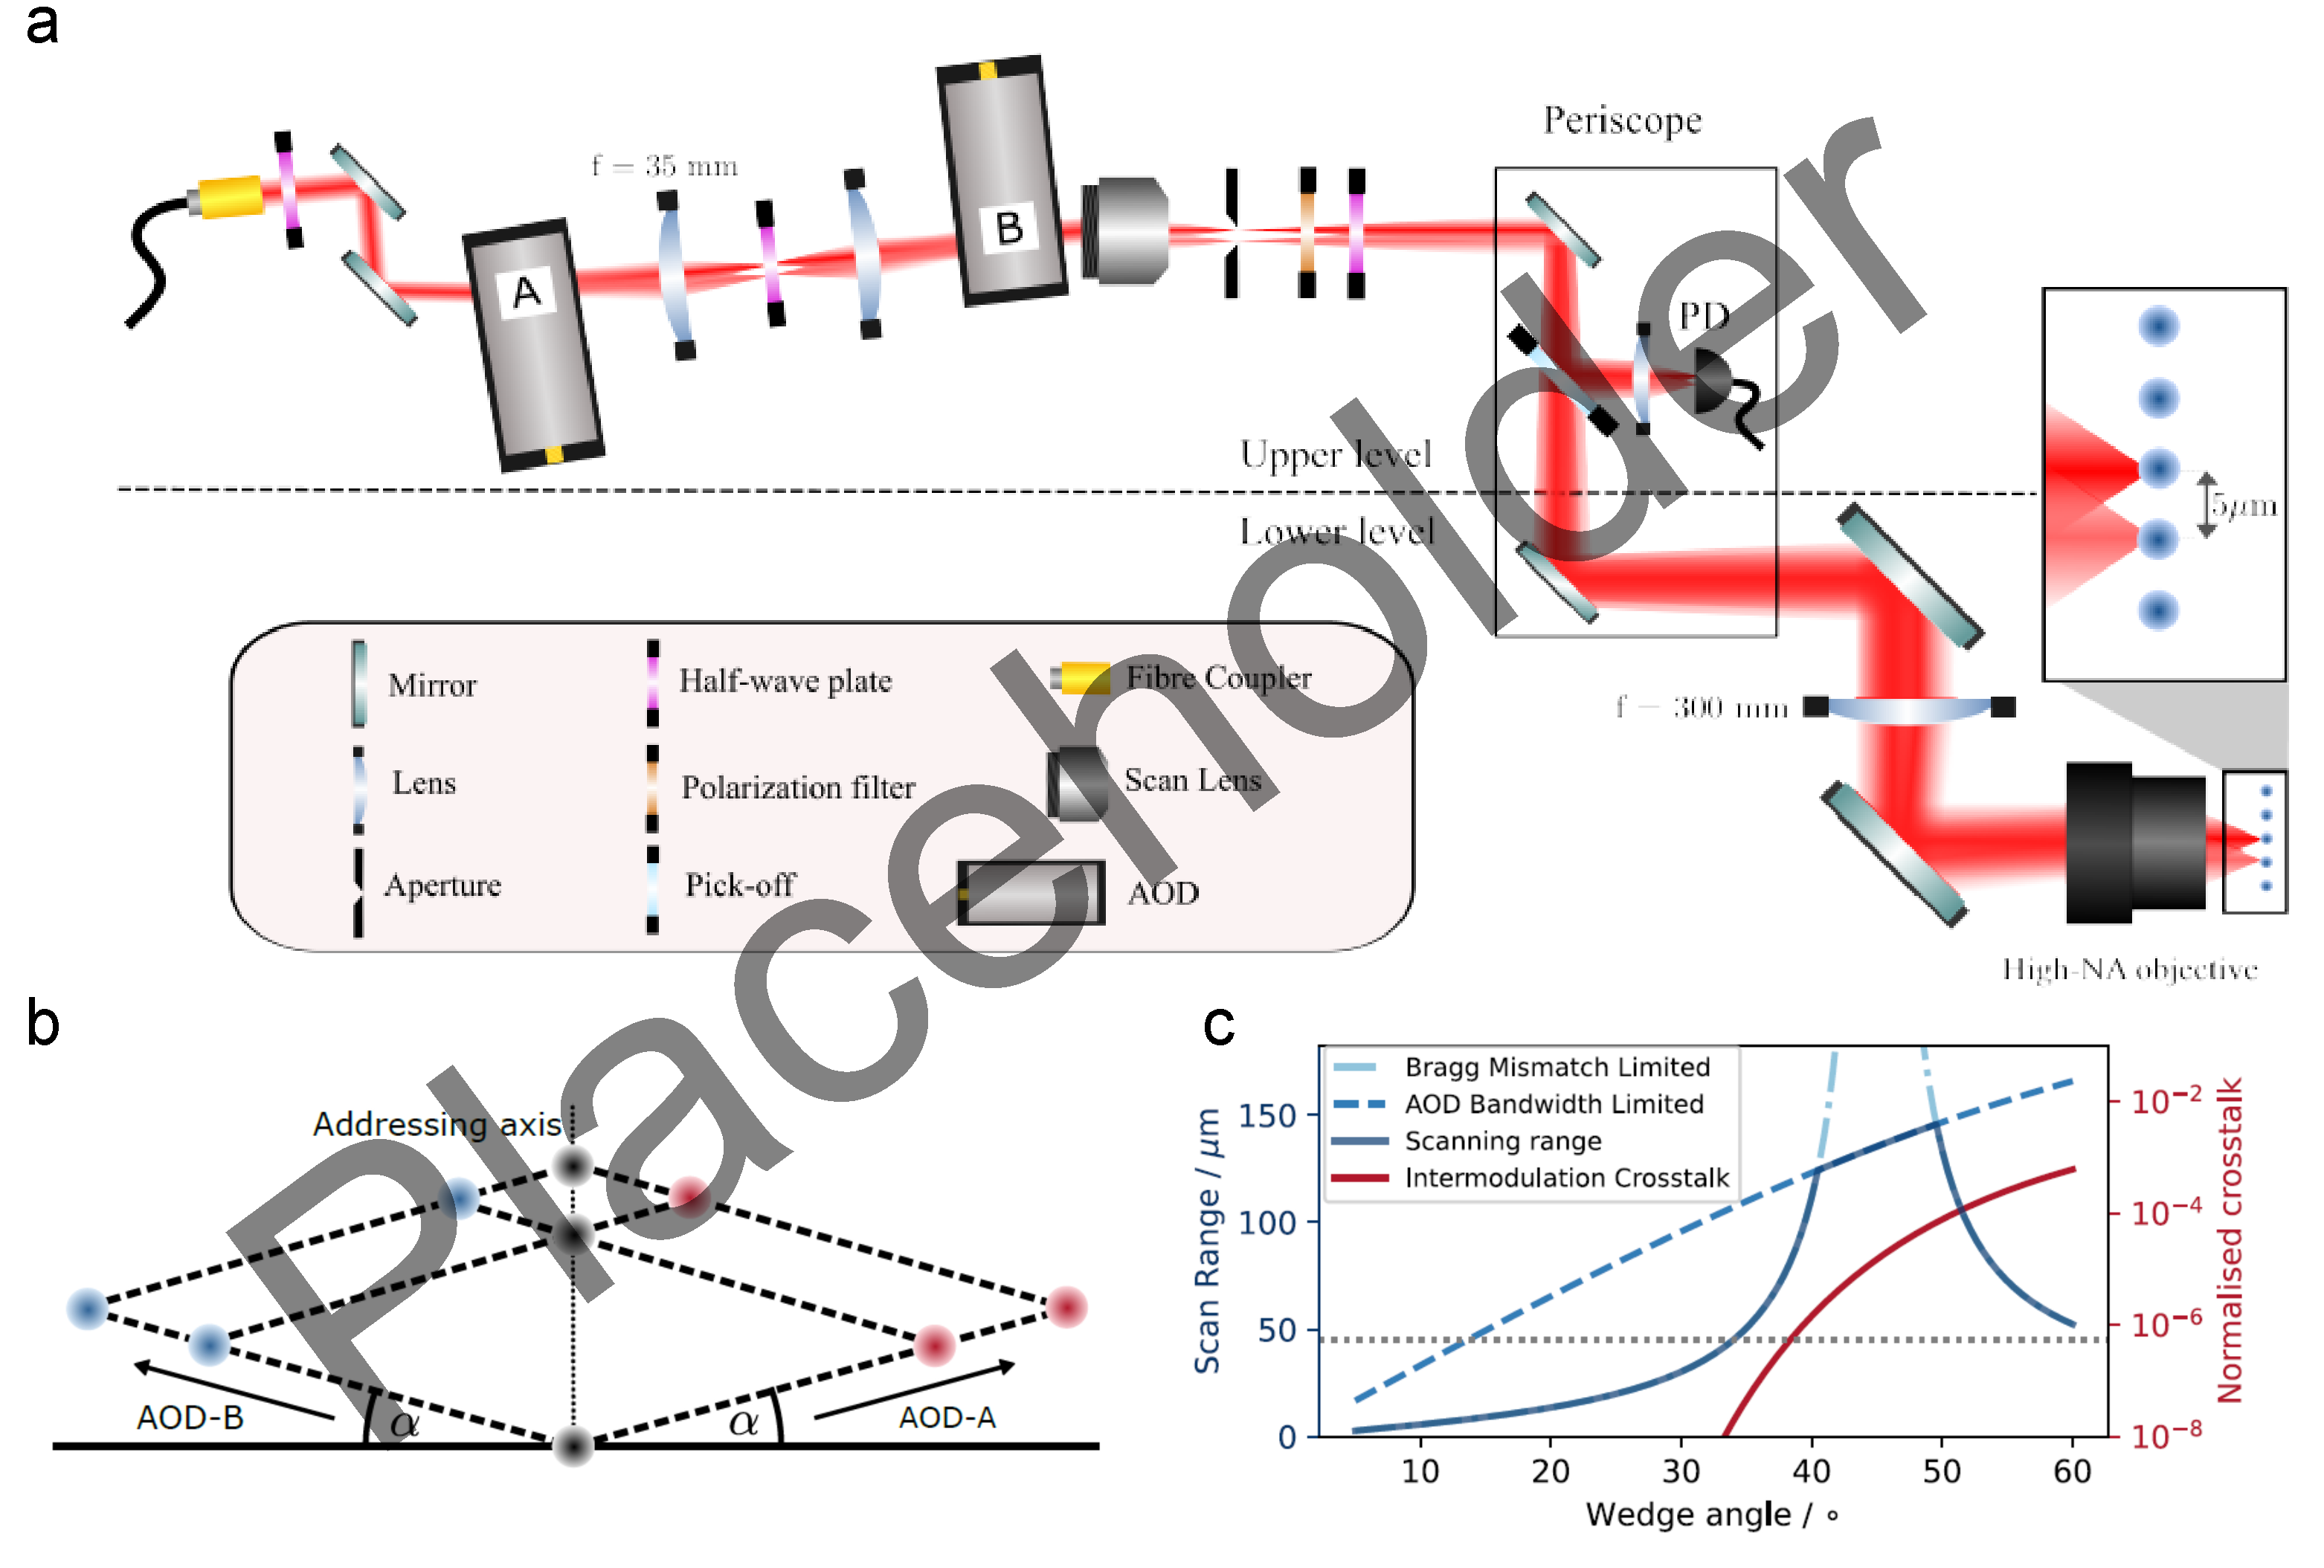
\includegraphics[width=\linewidth]{figures/pdf_figure/ch2/AOD_setup.pdf
            }
        \end{center}
        \caption{
            AOD setup
            }
        \label{fig:AOD}
    \end{figure}
% Main points:
    % The advantages of single addressing using AODs
        % Ion selectivity
        % High intensity electric field
    % single addressing system creating standing waves
    % render of single addressing system
% Pre reqs:
    % 729 system
    % High NA
    % Trap package
    % Motivation f
    Single ion addressing is a requirement for executing arbitrary circuits on a register of ion-qubits. Furthermore, it is advantageous to focus the optical drive onto the ion, increasing the intensity of light, and so driving faster gates.
    % Cross talk errors link here?
    A unique design feature of our system is the ability to produce an array of single ion addressing standing waves with individually contrallable spatial phase, thus enabling any-to-any connectivity for fast engangling gates based on the scheme demonstrated in Ref.~\cite{saner_breaking_2023}. \\
    %
    The design and construction of the single addressing system was led by Iver
    {\O}vergaard and, as of writing, has been in constant use in the experiment
    for around 1 year. Here we shall quote the design specification and relevant
    details of the single addressing system. In section~\ref{sec:Single
    Addressing char} we present the characterisation data upon installation.
    Further technical information can be found in IRO's Transfer
    report~\cite{oevergaard_transfer_2025}, availible upon request. \\
    %
    Multiple methods for single ion addressing have been developed in the ion
    trap community, including waveguide arrays~\cite{sotirova_high-fidelity_2024,
    mehta_integrated_2020}, micro-electronic-mechanical mirror arrays~\cite{crain_individual_2014, wang_high-fidelity_2020}, spatial-light-modulators~\cite{mazzanti_alignment_2024}, and
    acousto-optic deflectors~\cite{pogorelov_compact_2021, pernthaler_single_2019}. Each method has its own advantages and
    disadvantages in terms of speed, resolution, ease of integration, and
    scalability, and so choice of hardware is often a matter of experimental
    preference and constraints.
    We require:
    \begin{itemize}
        \item Addressing of up to two ions in a $\sim 10$ ion chain with low crosstalk to neighbouring ions.
        \item Fast reconfigureability of the beam position within a single experimental shot (i.e. between different gates within a single circuit execution).
        \item Good optical power efficiency to ensure high intensity electric fields at the ion. 
        \item Flexibility in beam positioning to allow for fine tuning of the overlap of two counterpropagating beams used to create the standing wave.
        \item Individual phase control of each addressed beam to stabilise the standing wave phase at the ion plane.
        \item Beam position stability to avoid power fluctuations.
        \item A compact design to fit within the magnetic shielded region of the experiment.
        \item Good telecentricity (fixed beam k-vector direction across the scanned area) to avoid unwanted travelling wave component in a standing wave gate scheme.
        \item Zero frequency shift of the beam at the ion plane.
    \end{itemize}
    Crossed Acousto-Optic Deflectors (cAODs) are a popular choice for single ion addressing, offering fast rise times ($\sim 10~\unit{\micro\second}$), and good resolution over a large scanning area ($\sim 500$ resolvable spots with $2^\circ$ angular range) with zero frequency shift along the addressing axis. AODs operate through the same mechanism as AOMs, but are optimised for beam deflection rather than frequency modulation. As an addressing system
    cAODs have poor scaling of power efficiency with the number of addressed spots, and so are not ideal for large scale systems. As we are interested in addressing $\leq 2$ ions at a time, this is not a significant issue for our system.\\
    %
    Figure~\ref{fig:AOD} (a) shows a schematic of the constructed addressing system. Due to space constraints within the magnetic shielded region, the optical elements are located on two height levels with a periscope steering the beam between them. The beam is delivered via single-mode polarisation maintaining fibre to the upper level where it is steered through the first AOD, with beam angle optimised for maximum diffraction efficiency into the $-1^{st}$ order. Two lenses\footnote{\todo{P/N}} in a 4f configuration re-image the deflection origin of the first AOD\footnote{\todo{P/N}} onto the second AOD with the second AOD angled for maximum diffraction efficiency into the $+1^{st}$ order. The cAOD arrangment is termed ``crossed'' as the second AOD is rotated by some angle $\alpha$ with respect to the first, so that the deflection from the second AOD has some orthogonal component to that of the first. When the two AODs are driven with RF tones of the same frequency, $f$, the high efficiency diffracted order combinations are: (0,0), ($-f$,0), (0,$+f$), ($-f$, $+f$). The last combination of $(-f, +f)$ has zero overall frequency shift yet retains some frequency dependent deflection angle, which is suitable for addressing ions in a 1D line. To translate this deflection angle into some physical displacement at the ion plane, a telecentric scanning lens\footnote{\todo{P/N}} is used. The telecentricity ensures that the beam k-vector direction is fixed across the scanned area, which is important for standing wave gate schemes to avoid unwanted travelling wave components. At the intermediate focus after the scanning lens, the unwanted orders are blocked by an adjustable slit aperture and the beam polarisation is cleaned and selected using a polarisation filter and half-wave plate. A plate beam splitter\footnote{\todo{P/N}} is used within the persicope to pick off $\sim 5\%$ of the light for monitoring on a photodiode\footnote{\todo{P/N}}, which is used in a feedback loop to stabilise the intensity at the ion plane (as discussed in section~\ref{sec:Intensity Stabilisation}). The scan lens, in combination with a relay lens, forms a beam expander to increase the beam NA for the final objective lens to focus to a beam waist of $\approx 1.5~\unit{\micro\meter}$ at the ion plane.
    %
    % Wedge angle
    % cAOD model numbers
    % Degrees of freedom for beam alignment
    Characterisation of the system (details given in section~\ref{sec:Single Addressing char}) showed that the addressing beam could be focused to a Gaussian waist of $1.50(1)~\unit{\micro\meter}$, measured by scanning a single trapped ion with Rabi experiments. The same beam was then tested in a five-ion chain, where the nearest-neighbour intensity crosstalk was measured to be $4.16(2)\times 10^{-4}$\todo{unit?}. 
    % Expected errors?
    % beam stability over time
    % Other mitigations for crosstalk?
    % How this links to k-copy RB?

    % TODO add section on Standing wave design and phase control?

\subsection{Global Addressing System}
\label{sec:Global Addressing System}
% Elliptical beam
The single addressing provides the utility of spatially selecting a few ions to
drive with the 729-nm light, however, the power efficiency scales as $O(n^2)$,
with $n$ being the number of addressed spots. As such, we limit the single addressing to simultaneously illuminate only one or two ions at a time. It is therefore convenient to also
have a global beam that has dimensions larger than the ion chain to address all the ions in parallel. This global branch is currently counterpropagating to the single addressing path, and shares the same optical path as the imaging system (see figure~\ref{fig:readout}). To increase
the beam intensity at the ions, the global branch uses an anamorphic prism
pair\footnote{\emph{ThorLabs} PS883-B} to elliptically shape the beam, with a
4:1 aspect ratio, with major axis along the ion chain direction.  The beam is focussed onto the ion plane using an $f=xx$ lens\footnote{\todo{P/N}}, resulting
in a major axis beam waist radius of $52(3)~\unit{\micro\meter}$\footnote{The
beam profile was measured by extracting per-ion Rabi frequencies while driving
on resonance quadrupole transitions (see section~\ref{sec:Single Qubit Gates}) and
assuming a Gaussian
cross section.}. As with the other beams directed to the ion, we use a final piezo controlled mirror\footnote{\emph{ThorLabs POLARIS}-K2S2P} for fine alignment and control when the MuMetal enclosure is closed.

\section{Control System}
% Main points:
    % Artiq and Sinara
    % FPGA control
    % Timing resolution
    \todo{Could tie up loose end here of control FPGA blocks.}

\section{Ion Loading}
% Main points:
    % Describe the ion loading process
    % Describe the atomic source oven
    % Describe the photoionisation process and lasers used
    Atoms are provided to the trapping region by heating Calcium flakes housed
    in a resistive tube oven with the oven mount shown in figure~\ref{fig:trap_package}. A
    thermocouple is tag welded onto the tube oven to provide a temperature reading
    for current feedback for fast stabilisation to the target temperature of $\simeq
    200^\circ\mathrm{C}$. A steady state of $\simeq 2~\unit{A}$
    across the $0.5~\unit{\ohm}$ load of the oven tube is required to maintain $200^\circ\mathrm{C}$. The tube oven has a
    pinhole that is aligned to the ion flux aperture, visible in
    figure~\ref{fig:trap_package} with atom flux shown in green, and the atomic shield pinhole shown in
    figure~\ref{fig:trap}. These apertures were included in the design to
    improve the operational lifetime of the trap by ensuring neutral Calcium metal cannot
    accumulate on the trap surface and cause shorts between RF, ground, and DC
    electrodes. The aperture design \emph{luckily} failed. It failed as we
    observe atomic flux at all electrode locations suggesting the aperture is
    too large. It was \emph{lucky} as the planned trapping region of \emph{dc10} became
    non-viable after electrode \emph{Fr dc11} developed a continuity fault. As such, ions are loaded at \emph{dc5}.\\
    The neutral atom flux is ionised using a two-step photoionisation
    scheme~\cite{lucas_isotope-selective_2004} that can selectively load the desired isotope of Calcium.
    Natural abundance Calcium, with typical isotope proportions of
    $96.9\%:\mathrm{^{40}Ca},~2.09\%:\mathrm{^{44}Ca},~0.647\%:\mathrm{^{43}Ca}$~\cite{lucas_isotope-selective_2004}, was appropriate as we aim to exclusively load \ca.
    The first stage involves a frequency stabilised 423-nm beam
    that couples the $4\mathrm{s}^2\rightarrow 4\mathrm{s}4\mathrm{p}$ transition in neutral calcium. The natural linewidth of this transition ($\simeq 35~\unit{\mega\hertz}$) is much smaller than the isotope shifts between abundant isotopes of Calcium (typically $>100~\unit{\mega\hertz}$ shifts), as such, through frequency selectivity, only the desired isotope can be excited. 
    The second ionisation stage couples $4\mathrm{s}4\mathrm{p}\rightarrow \mathrm{continuum}$ through
    a 373-nm UV laser source (although the exact wavelength does not matter as
    long as <389.8-nm).
    We practically see no loading of other
    Calcium isotopes, and only see rare non-fluorescent ions (once every few
    weeks) after collisions with residual gas (we suspect this is
    $\mathrm{CaH}^+$). \\
    The 373-nm laser causes charge build-up on the trap electrodes, which can
    affect the trapping potential, and so 
    a physical shutter, controlled by a TTL signal, is used to block
    the beam when not actively loading ions.\\
